\documentclass[a4paper, 12pt, twoside]{article}


%------------------------------------------------------------------------
%
% Author                :   arcln production
% Last modification     :   2023.1.12
%
%------------------------------------------------------------------------


%------ini
\usepackage[utf8]{inputenc}
\usepackage[T1]{fontenc}
\usepackage[french]{babel}
%\usepackage[english]{babel}


%------geometry
\usepackage[textheight=700pt, textwidth=500pt]{geometry}


%------color
\usepackage{xcolor}
\definecolor{0010A1}{HTML}{0010A1}
\definecolor{00f}{HTML}{0000ff}
\definecolor{0ff}{HTML}{00ffff}
\definecolor{656565}{HTML}{656565}

%\renewcommand{\emph}{\textcolor{0010A1}}
%\renewcommand{\em}{\color{0010A1}}

\newcommand{\Emph}{\textcolor{0010A1}}

\newcommand{\strong}[1]{\textcolor{0010A1}{\bf #1}}
\newcommand{\st}{\color{0010A1}\bf}


%------Code highlighting
%---listings
\usepackage{listings}

\definecolor{cbg}{HTML}{272822}
\definecolor{cfg}{HTML}{ececec}
\definecolor{ccomment}{HTML}{686c58}
\definecolor{ckw}{HTML}{f92672}
\definecolor{cstring}{HTML}{e6db72}
\definecolor{cstringlight}{HTML}{98980f}
\definecolor{lightwhite}{HTML}{fafafa}

\lstdefinestyle{DarkCodeStyle}{
    backgroundcolor=\color{cbg},
    commentstyle=\itshape\color{ccomment},
    keywordstyle=\color{ckw},
    numberstyle=\tiny\color{cbg},
    stringstyle=\color{cstring},
    basicstyle=\ttfamily\footnotesize\color{cfg},
    breakatwhitespace=false,
    breaklines=true,
    captionpos=b,
    keepspaces=true,
    numbers=left,
    numbersep=5pt,
    showspaces=false,
    showstringspaces=false,
    showtabs=false,
    tabsize=4,
    xleftmargin=\leftskip
}

\lstdefinestyle{LightCodeStyle}{
    backgroundcolor=\color{lightwhite},
    commentstyle=\itshape\color{ccomment},
    keywordstyle=\color{ckw},
    numberstyle=\tiny\color{cbg},
    stringstyle=\color{cstringlight},
    basicstyle=\ttfamily\footnotesize\color{cbg},
    breakatwhitespace=false,
    breaklines=true,
    captionpos=b,
    keepspaces=true,
    numbers=left,
    numbersep=10pt,
    showspaces=false,
    showstringspaces=false,
    showtabs=false,
    tabsize=4,
    frame=L,
    xleftmargin=\leftskip
}

%\lstset{style=DarkCodeStyle}
\lstset{style=LightCodeStyle}
%Usage : \begin{lstlisting}[language=Caml, xleftmargin=xpt] ... \end{lstlisting}


%---Algorithm
\usepackage[linesnumbered,ruled,vlined]{algorithm2e}
\SetKwInput{KwInput}{Input}
\SetKwInput{KwOutput}{Output}

\SetKwProg{Fn}{Function}{:}{}
\SetKw{KwPrint}{Print}

\newcommand\commfont[1]{\textit{\texttt{\textcolor{656565}{#1}}}}
\SetCommentSty{commfont}
\SetProgSty{texttt}
\SetArgSty{textnormal}
\SetFuncArgSty{textnormal}
%\SetProgArgSty{texttt}

\newenvironment{indalgo}[2][H]{
    \begin{algoBox}
        \begin{algorithm}[#1]
            \caption{#2}
}
{
        \end{algorithm}
    \end{algoBox}
}


%---tcolorbox
\usepackage[many]{tcolorbox}
\DeclareTColorBox{emphBox}{O{black}O{lightwhite}}{
    breakable,
    outer arc=0pt,
    arc=0pt,
    top=0pt,
    toprule=-.5pt,
    right=0pt,
    rightrule=-.5pt,
    bottom=0pt,
    bottomrule=-.5pt,
    colframe=#1,
    colback=#2,
    enlarge left by=10pt,
    width=\linewidth-\leftskip-10pt,
}

\DeclareTColorBox{algoBox}{O{black}O{lightwhite}}{
    breakable,
    arc=0pt,
    top=0pt,
    toprule=-.5pt,
    right=0pt,
    rightrule=-.5pt,
    bottom=0pt,
    bottomrule=-.5pt,
    left=0pt,
    leftrule=-.5pt,
    colframe=#1,
    colback=#2,
    width=\linewidth-\leftskip-10pt,
}


%-------make the table of content clickable
\usepackage{hyperref}
\hypersetup{
    colorlinks,
    citecolor=black,
    filecolor=black,
    linkcolor=black,
    urlcolor=black
}


%------pictures
\usepackage{graphicx}
%\usepackage{wrapfig}

\usepackage{tikz}
%\usetikzlibrary{babel}             %Uncomment this to use circuitikz
%\usetikzlibrary{shapes.geometric}  % To draw triangles in trees
%\usepackage{circuitikz}            %Electrical circuits drawing


%------tabular
%\usepackage{color}
%\usepackage{colortbl}
%\usepackage{multirow}


%------Mathpartir (inference rules)
\usepackage{mathpartir}


%------Physics
%---Packages
%\usepackage[version=4]{mhchem} %$\ce{NO4^2-}$

%---Commands
\newcommand{\link}[2]{\mathrm{#1} \! - \! \mathrm{#2}}
\newcommand{\pt}[1]{\cdot 10^{#1}} % Power of ten
\newcommand{\dt}[2][t]{\dfrac{\mathrm d #2}{\mathrm d #1}} % Derivative


%------math
%---Packages
%\usepackage{textcomp}
%\usepackage{amsmath}
\usepackage{amssymb}
\usepackage{mathtools} % For abs
\usepackage{stmaryrd} %for \llbracket and \rrbracket
\usepackage{mathrsfs} %for \mathscr{x} (different from \mathcal{x})

%---Commands
%-Sets
\newcommand{\N}{\mathbb{N}} %set N
\newcommand{\Z}{\mathbb{Z}} %set Z
\newcommand{\Q}{\mathbb{Q}} %set Q
\newcommand{\R}{\mathbb{R}} %set R
\newcommand{\C}{\mathbb{C}} %set C
\newcommand{\U}{\mathbb{U}} %set U
\newcommand{\seg}[2]{\left[ #1\ ;\ #2 \right]}
\newcommand{\nset}[2]{\left\llbracket #1\ ;\ #2 \right\rrbracket}

%-Exponantial / complexs
\newcommand{\e}{\mathrm{e}}
\newcommand{\cj}[1]{\overline{#1}} %overline for the conjugate.

%-Vectors
\newcommand{\vect}{\overrightarrow}
\newcommand{\veco}[3]{\displaystyle \vect{#1}\binom{#2}{#3}} %vector + coord

%-Limits
\newcommand{\lm}[2][{}]{\lim\limits_{\substack{#2 \\ #1}}} %$\lm{x \to a} f$ or $\lm[x < a]{x \to a} f$
\newcommand{\Lm}[3][{}]{\lm[#1]{#2} \left( #3 \right)} %$\Lm{x \to a}{f}$ or $\Lm[x < a]{x \to a}{f}$
\newcommand{\tendsto}[1]{\xrightarrow[#1]{}}

%-Integral
\newcommand{\dint}[4][x]{\displaystyle \int_{#2}^{#3} #4 \mathrm{d} #1} %$\dint{a}{b}{f(x)}$ or $\dint[t]{a}{b}{f(t)}$

%-left right
\newcommand{\lr}[1]{\left( #1 \right)}
\newcommand{\lrb}[1]{\left[ #1 \right]}
\newcommand{\lrbb}[1]{\left\llbracket #1 \right\rrbracket}
\newcommand{\set}[1]{\left\{ #1 \right\}}
\newcommand{\abs}[1]{\left\lvert #1 \right\rvert}
\newcommand{\ceil}[1]{\left\lceil #1 \right\rceil}
\newcommand{\floor}[1]{\left\lfloor #1 \right\rfloor}
\newcommand{\lrangle}[1]{\left\langle #1 \right\rangle}

%-Others
\newcommand{\para}{\ /\!/\ } %//
\newcommand{\ssi}{\ \Leftrightarrow \ }
\newcommand{\eqsys}[2]{\begin{cases} #1 \\ #2 \end{cases}}

\newcommand{\med}[2]{\mathrm{med} \left[ #1\ ;\ #2 \right]}  %$\med{A}{B} -> med[A ; B]$
\newcommand{\Circ}[2]{\mathscr{C}_{#1, #2}}

\renewcommand{\le}{\leqslant}
\renewcommand{\ge}{\geqslant}

\newcommand{\oboxed}[1]{\textcolor{0010A1}{\boxed{\textcolor{black}{#1}}}} %orange boxed

\newcommand{\rboxed}[1]{\begin{array}{|c} \hline #1 \\ \hline \end{array}} %boxed with right opened
\newcommand{\lboxed}[1]{\begin{array}{c|} \hline #1 \\ \hline \end{array}} %boxed with left opened

\newcommand{\orboxed}[1]{\textcolor{0010A1}{\rboxed{\textcolor{black}{#1}}}} %orange right boxed
\newcommand{\olboxed}[1]{\textcolor{0010A1}{\lboxed{\textcolor{black}{#1}}}} %orange left boxed


%------commands
%---to quote
\newcommand{\simplecit}[1]{\guillemotleft$\;$#1$\;$\guillemotright}
\newcommand{\cit}[1]{\simplecit{\textcolor{656565}{#1}}}
\newcommand{\quo}[1]{\cit{\it #1}}

%---to indent
\newcommand{\ind}[1][20pt]{\advance\leftskip + #1}
\newcommand{\deind}[1][20pt]{\advance\leftskip - #1}

%---to indent a text
\newcommand{\indented}[2][20pt]{\par \ind[#1] #2 \par \deind[#1]}
\newenvironment{indt}[2][20pt]{#2 \par \ind[#1]}{\par \deind} %Titled indented env

%---title
\newcommand{\thetitle}[2]{\begin{center}\textbf{{\LARGE \underline{\Emph{#1} :}} {\Large #2}}\end{center}}

%---Maths environments
%-Proofs
\newenvironment{proof}[1][{}]{\begin{indt}{$\square$ #1}}{$\blacksquare$ \end{indt}}

%-Maths parts (proposition, definition, ...)
\newenvironment{mathpart}[1]{\begin{indt}{\boxed{\text{\textbf{#1}}}}}{\end{indt}}
\newenvironment{mathbox}[1]{\boxed{\text{\textbf{#1}}}\begin{emphBox}}{\end{emphBox}}
\newenvironment{mathul}[1]{\begin{indt}{\underline{\textbf{#1}}}}{\end{indt}}

\newenvironment{theo}{\begin{mathpart}{Théorème}}{\end{mathpart}}
\newenvironment{Theo}{\begin{mathbox}{Théorème}}{\end{mathbox}}

\newenvironment{prop}{\begin{mathpart}{Proposition}}{\end{mathpart}}
\newenvironment{Prop}{\begin{mathbox}{Proposition}}{\end{mathbox}}
\newenvironment{props}{\begin{mathpart}{Propriétés}}{\end{mathpart}}

\newenvironment{defi}{\begin{mathpart}{Définition}}{\end{mathpart}}
\newenvironment{meth}{\begin{mathpart}{Méthode}}{\end{mathpart}}

\newenvironment{Rq}{\begin{mathul}{Remarque :}}{\end{mathul}}
\newenvironment{Rqs}{\begin{mathul}{Remarques :}}{\end{mathul}}

\newenvironment{Ex}{\begin{mathul}{Exemple :}}{\end{mathul}}
\newenvironment{Exs}{\begin{mathul}{Exemples :}}{\end{mathul}}


%------Sections
% To change section numbering :
% \renewcommand\thesection{\Roman{section}}
% \renewcommand\thesubsection{\arabic{subsection})}
% \renewcommand\thesubsubsection{\textit \alph{subsubsection})}

% To start numbering from 0
% \setcounter{section}{-1}


%------page style
\usepackage{fancyhdr}
\usepackage{lastpage}

\setlength{\headheight}{18pt}
\setlength{\footskip}{50pt}

\pagestyle{fancy}
\fancyhf{}
\fancyhead[LE, RO]{\textit{\textcolor{black}{\today}}}
\fancyhead[RE, LO]{\large{\textsl{\Emph{\texttt{Rapport de Soutenance 1}}}}}

\fancyfoot[RO, LE]{\textit{\texttt{\textcolor{black}{Page \thepage /}\pageref{LastPage}}}}
\fancyfoot[LO, RE]{
\includegraphics[scale=0.12]{arcln}}


%------init lengths
\setlength{\parindent}{0pt} %To avoid using \noindent everywhere.
\setlength{\parskip}{3pt}

% Mise en page française
\usepackage[utf8]{inputenc}
\usepackage[french]{babel}
\usepackage{geometry}

% Import d'images, couleurs
\usepackage{graphicx,color}

\usepackage{lipsum}

\newcommand{\hsp}{\hspace{20pt}}
\newcommand{\HRule}{\rule{\linewidth}{0.5mm}}

%---------------------------------Begin Document
\begin{document}

    
\begin{titlepage}
  \begin{sffamily}
  \begin{center}

  
    
\includegraphics[scale=0.3]{logo}~\\[1.5cm]

    \textsc{\LARGE EPITA Rennes}\\[0.5cm]

    % Titre
    \textsc{\Large RAPPORT DU PROJET S2}\\[1.5cm]

    \HRule \\[0.4cm]
     { \huge \bfseries  A Slime's Journey \\[0.4cm] }

    \HRule \\[2cm]
    
\includegraphics[scale=0.4]{arcln}
     \\[0.5cm]
    %\textsc{\Large ARCLN}\\[1.5cm]

    % Membres
    \begin{minipage}{0.4\textwidth}
      \begin{flushleft} \large
        Alexis LE GALL\\
        Enzo JUHEL\\
      \end{flushleft}
    \end{minipage}
    \begin{minipage}{0.4\textwidth}
      \begin{flushright} \large
        Maxime DOUILLARD\\
        Omid SHEIBANIFAR\\
      \end{flushright}
    \end{minipage}

    \vfill

  \end{center}
  \end{sffamily}
\end{titlepage}


    \tableofcontents
    \newpage

    \begin{indt}{\section{Introduction}}
        “A Slime's Journey” est un jeu développé par la compagnie ARCLN prod. Ce projet est réalisé dans le cadre du projet du second semestre d'Epita. Il est réalisé par Alexis Le Gall, Enzo Juhel, Omid Sheibanifar et Maxime Douillard. Ce jeu est un platformer 2D reliant histoire et énigmes et se déroule dans un univers médiéval.

        Actuellement, le joueur peut prendre le contrôle d'un slime, une sorte de blob qui peut se déplacer avec des petits sauts. De plus, ce slime est capable de sauter, que ce soit pour atteindre d'autres plateformes mais aussi pour attaquer les ennemis en leur saute par dessus. De plus, le jeu arbore un style médiéval et pixelisé. Ce jeu peut se jouer en coopération par le biais d'un mode multijoueur en ligne. Cela permet de découvrir ou redécouvrir le jeu avec un autre joueur. Malgré la présence d'un second joueur, la difficulté des niveaux ne change pas. Comme le premier joueur, le deuxième joueur peut incarner un slime qui possède les mêmes capacités que le premier joueur.

        Dans ce document, nous verrons, tout d'abord, un ensemble des points pertinents du jeu, puis une chronologie des avancées de chacuns restitués personnellement. Enfin une comparaison en rétrospective de ce que nous avions prévu pour la première soutenance, suivi de l'annexe comprenant les ressources utiles à la compréhension de l'avancée du projet.
    \end{indt}
    
    \begin{indt}{\section{Résumé cahier des charges}}
        Pour ce projet, notre entreprise a décidé de créer un jeu de plateforme en 2D. Inspiré de divers jeux vidéo, notre jeu comportera certaines ressemblances avec eux mais aussi certains des points de divergences. Le joueur prendra le contrôle d'un slime, une sorte de blob qui peut se déplacer avec des petits sauts. En multijoueur, les joueurs pourront vaincre des monstres se trouvant sur leur passage à l'aide d'équipement ramassé au préalable durant les précédents niveaux, ou à l'aide de leurs capacités temporaires.
    
        \begin{center}
            \begin{tabular}{|c|c|c|c|c|}
                \hline
                & Alexis & Enzo & Maxime & Omid
                \\
                \hline
                Développement & Participant & Participant & Responsable & Suppléant
                \\
                \hline
                Communication & Suppléant & & Responsable &
                \\
                \hline
                Design & & Responsable & Suppléant &
                \\
                \hline
                Audio & Suppléant & & & Responsable
                \\
                \hline
                IA & Responsable & & & Suppléant
                \\
                \hline
                Réseau & Responsable & Suppléant & Participant & Participant
                \\
                \hline
                Rédaction & Participant & Responsable & Participant & Suppléant
                \\
                \hline
            \end{tabular}
        \end{center}
    \end{indt}

    \newpage
    
    \begin{indt}{\section{Chronologie des avancements personnels}}
        \begin{indt}{\subsection{Enzo}}
            Lors de notre première réunion concernant ce tout premier projet de groupe, nous étions à la recherche d'une idée de jeu. Ce projet de second semestre est pour nous une très grande opportunité de pouvoir mettre en œuvre les compétences que nous avons acquises depuis le début de nos études supérieures. Nous avions eu comme première approche d'idée  de jeu de faire un FPS (jeu de tir à la première personne), cependant, il s'est avéré que cela nous paraissait, à tous, assez compliqué de faire quelque chose de réaliste. Nous avons donc eu une conversation ou tout le monde a énoncé des idées de jeux, tous plus originaux les uns que les autres. Malgré tout, nous nous sommes mis d'accord sur un jeu qui a pour protagoniste un slime, une sorte de pâte gluante et élastique, qui pourrait changer de forme selon son environnement extérieur et ainsi acquérir de nouvelles capacités afin de surmonter les obstacles. Ainsi, notre jeu sera, alors, un jeu de plateforme avec des combats contre des boss, il comportera aussi des énigmes ainsi que des transformations.

            Par la suite, nous avions alors l'idée du jeu mais cependant, nous n'avions pas encore trouvé le but et la finalité de notre jeu. Nous avons donc décidé d'avoir pour objectif un château qui serait visible depuis le début du jeu et qui se rapprocherait à chaque niveau passé. Après avoir fait tout cela, il nous manquait encore le plus important, le nom du jeu. Nous en avons discuté longuement puis nous avons réussi à nous mettre d'accord sur “A Slime's Journey”.
        	
            Nous avions alors le choix de comment se partager le projet. Cette partie fut assez rapidement résolue car nous avons décidé de passer par GitHub après les conseils de personnes des années précédentes. Nous avons donc créé un repo. Ce repo nous a permis de toujours travailler sur une version actuelle du jeu. Nous avons quand même rencontré quelques difficultés lors de rassembler le travail ensemble, nous avons dû revenir sur des versions précédentes du jeu ce qui nous a fait perdre un peu de temps.
        	
            De prime abord, nous avions décidé que le jeu aurait un style inspiré des cartoons, comme le jeu Cuphead qui est un jeu de plateforme sorti assez récemment.
            
            \begin{center}
                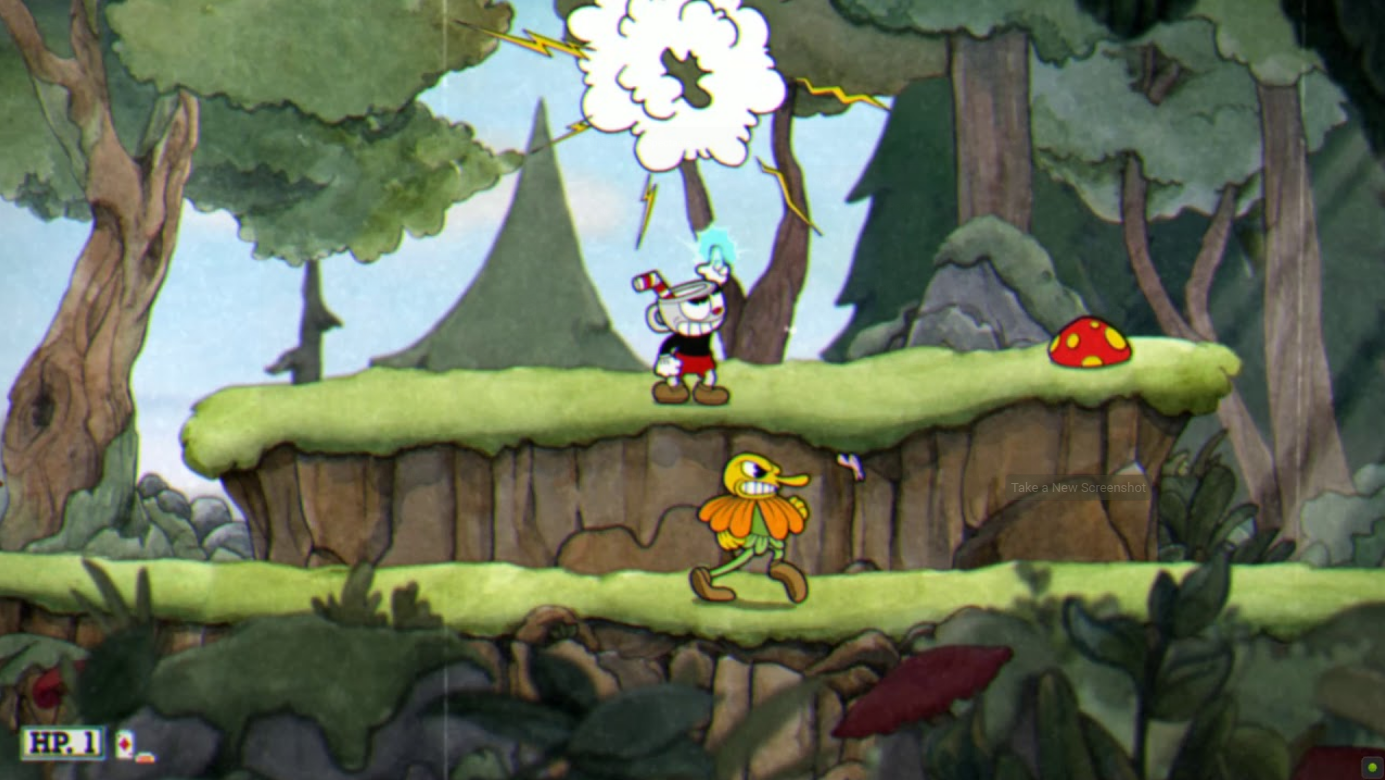
\includegraphics[width=0.8\linewidth]{Cuphead.png}
            \end{center}

            Cependant, lors de la réalisation des premiers croquis et dessins des personnages ainsi que des décors, nous nous sommes rendu compte que cela aller être plutôt compliqué à réaliser après avoir réalisé les dessins des éléments du jeu dont le slime ci-dessous. Nous nous sommes donc concertés et avons décidé de nous mettre d'accord pour aborder un style “Pixel Art” à la place. En effet, ce type de graphisme est bien plus simple à réaliser.

            \begin{center}
                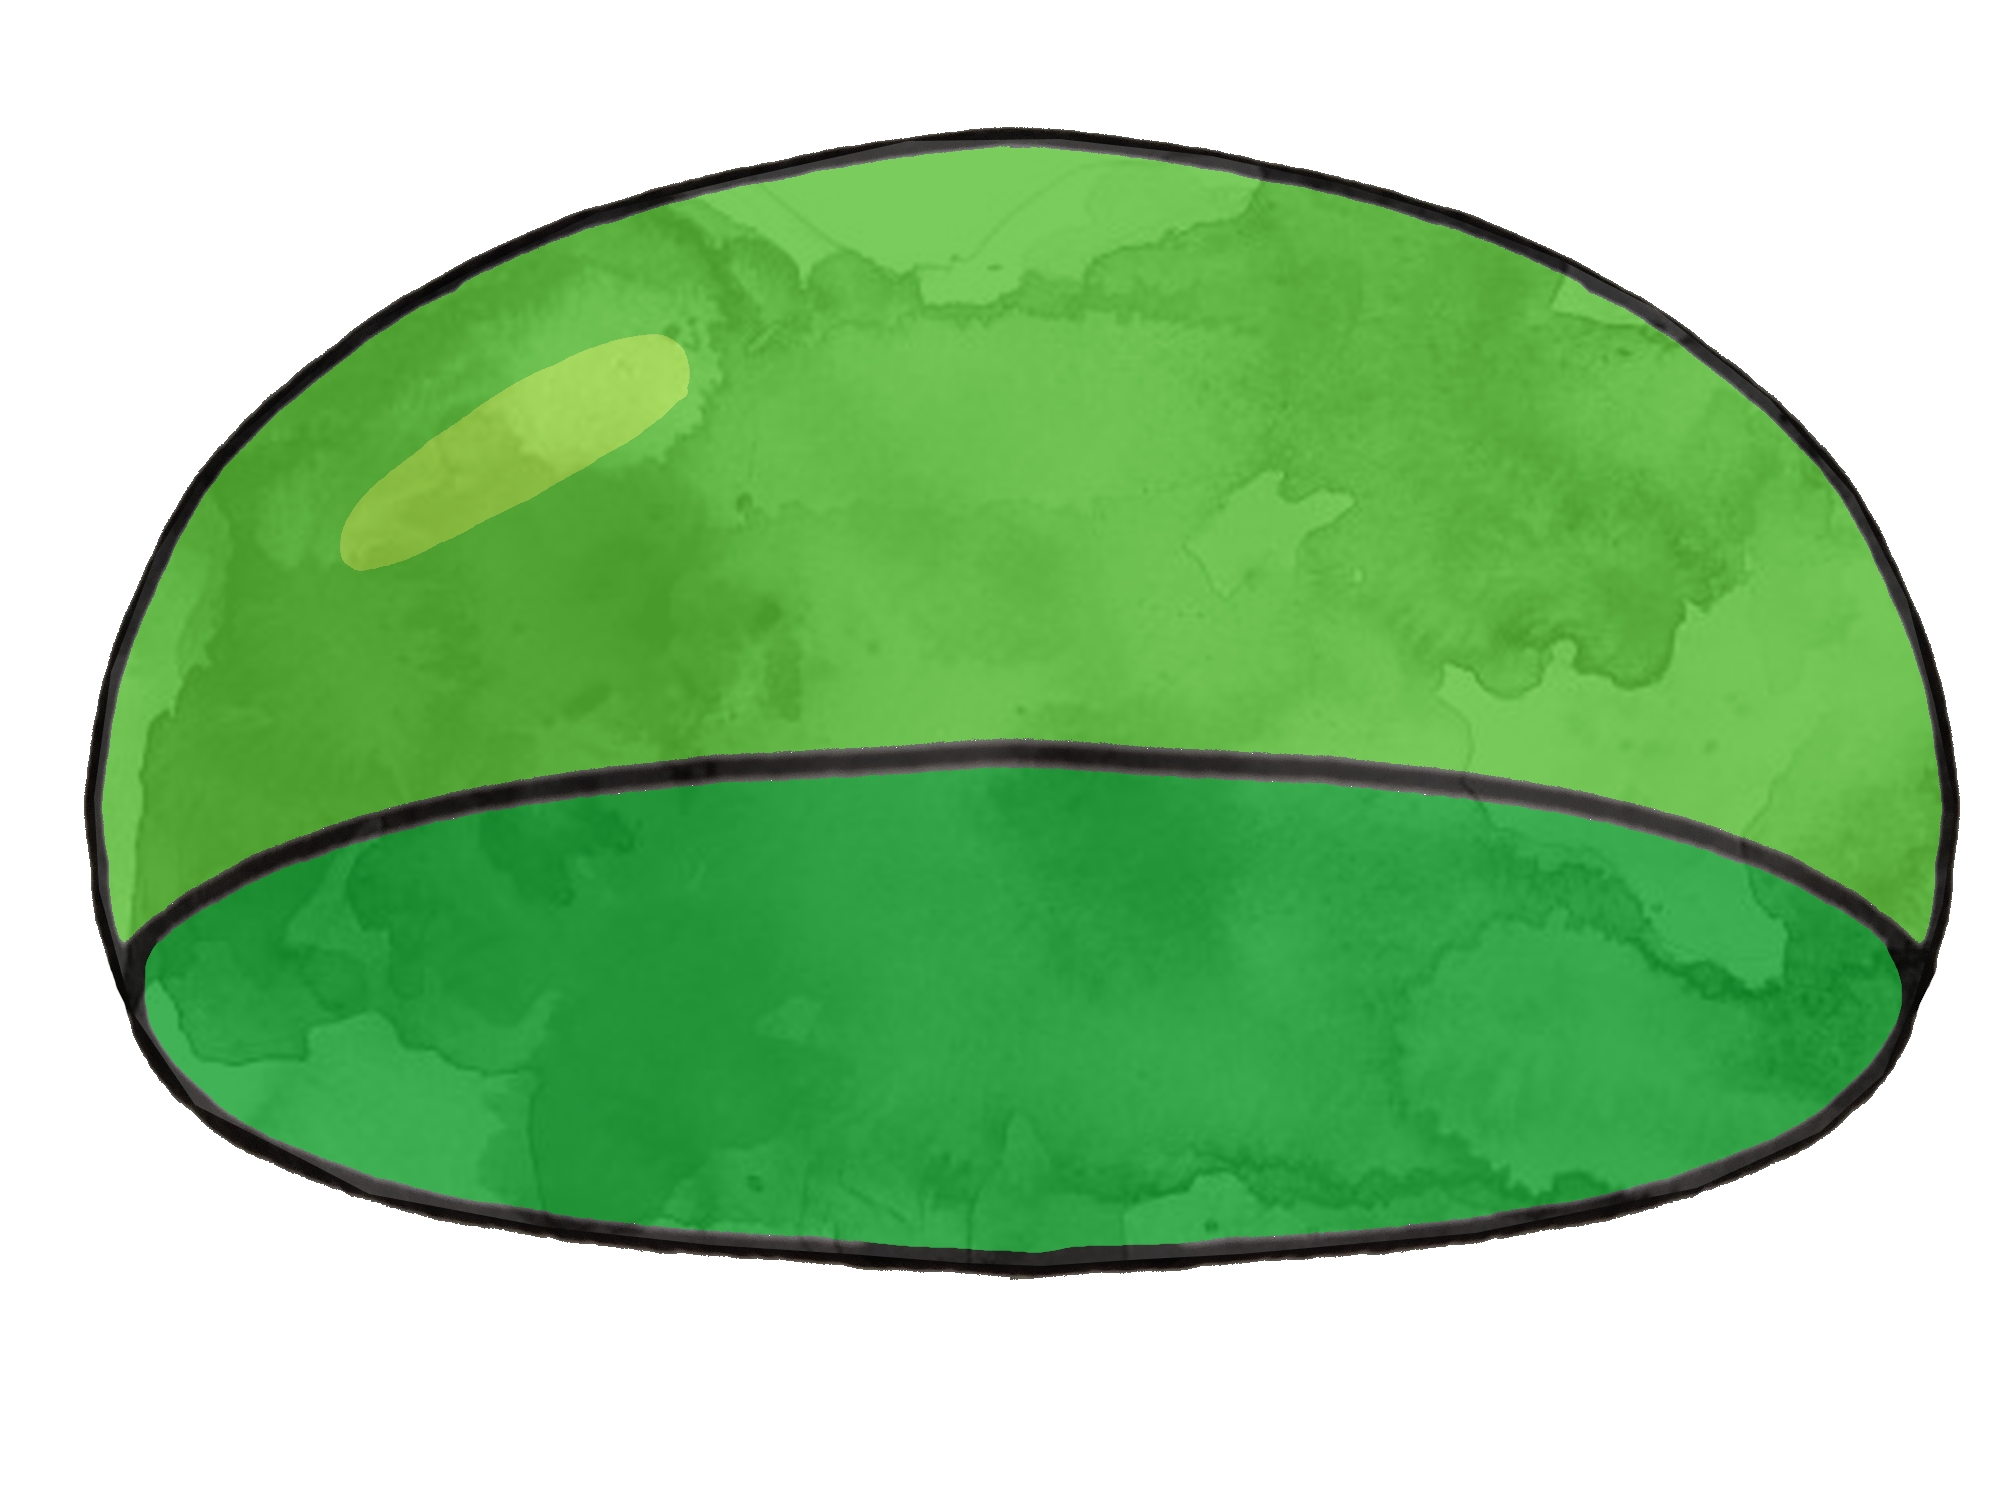
\includegraphics[width=0.2\linewidth]{Slime.jpg}
            \end{center}

            Une tâche qui m'a été assignée fut de créer le menu principal. La première version de ce menu comportait une interface avec la possibilité d'avoir 3 sauvegardes, 3 parties en lignes que l'on peut rejoindre ainsi que la possibilité de créer une partie en multijoueur. Cependant, de nombreux problèmes dut à la connexion en ligne, nous ont contraints à recommencer le projet depuis le départ . Néanmoins, cela fut pour le mieux car cette fois, nous avions les connaissances pour pouvoir le faire correctement. Cela nous a permis de faire une interface de menu bien plus aérée, plaisante à regarder, de plus elle est beaucoup plus en lien avec le style de notre jeu.

            \begin{figure}
                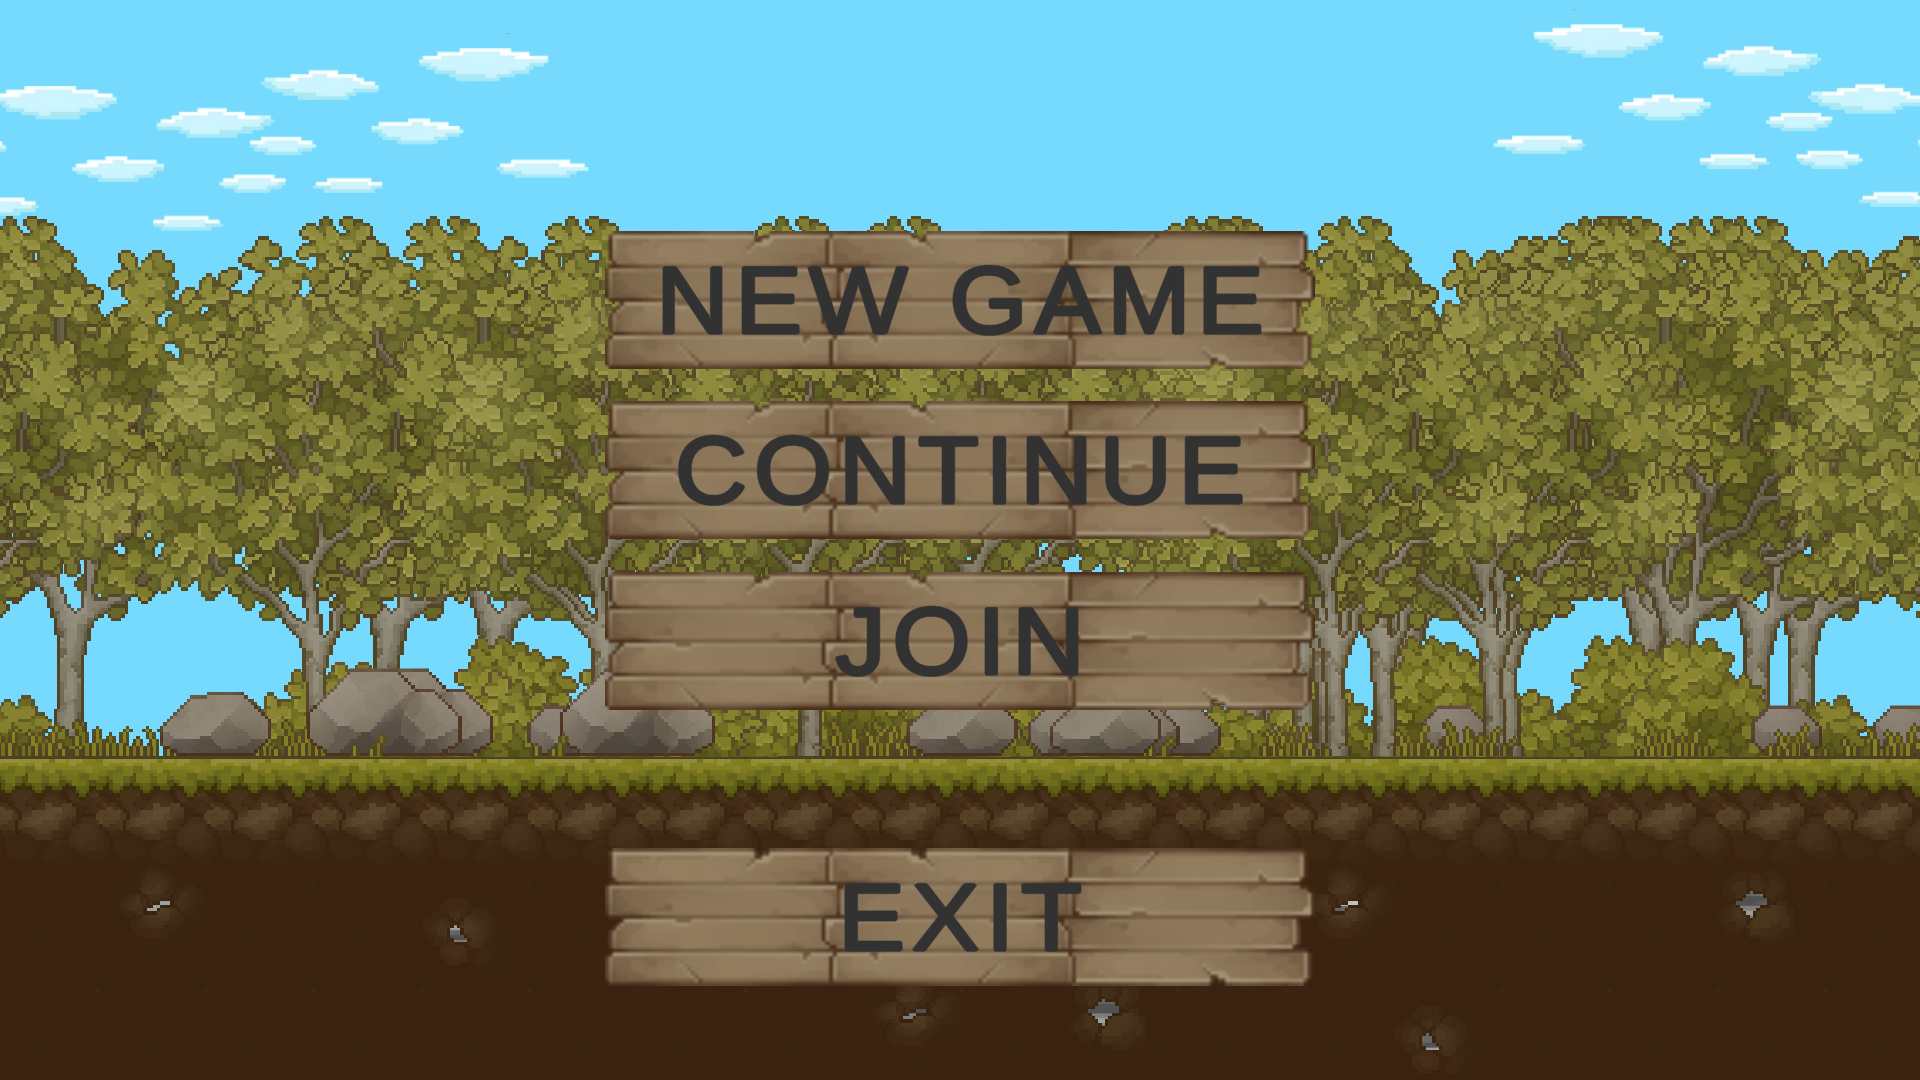
\includegraphics[width=0.49\linewidth]{MMV11.png}\hfill \hfill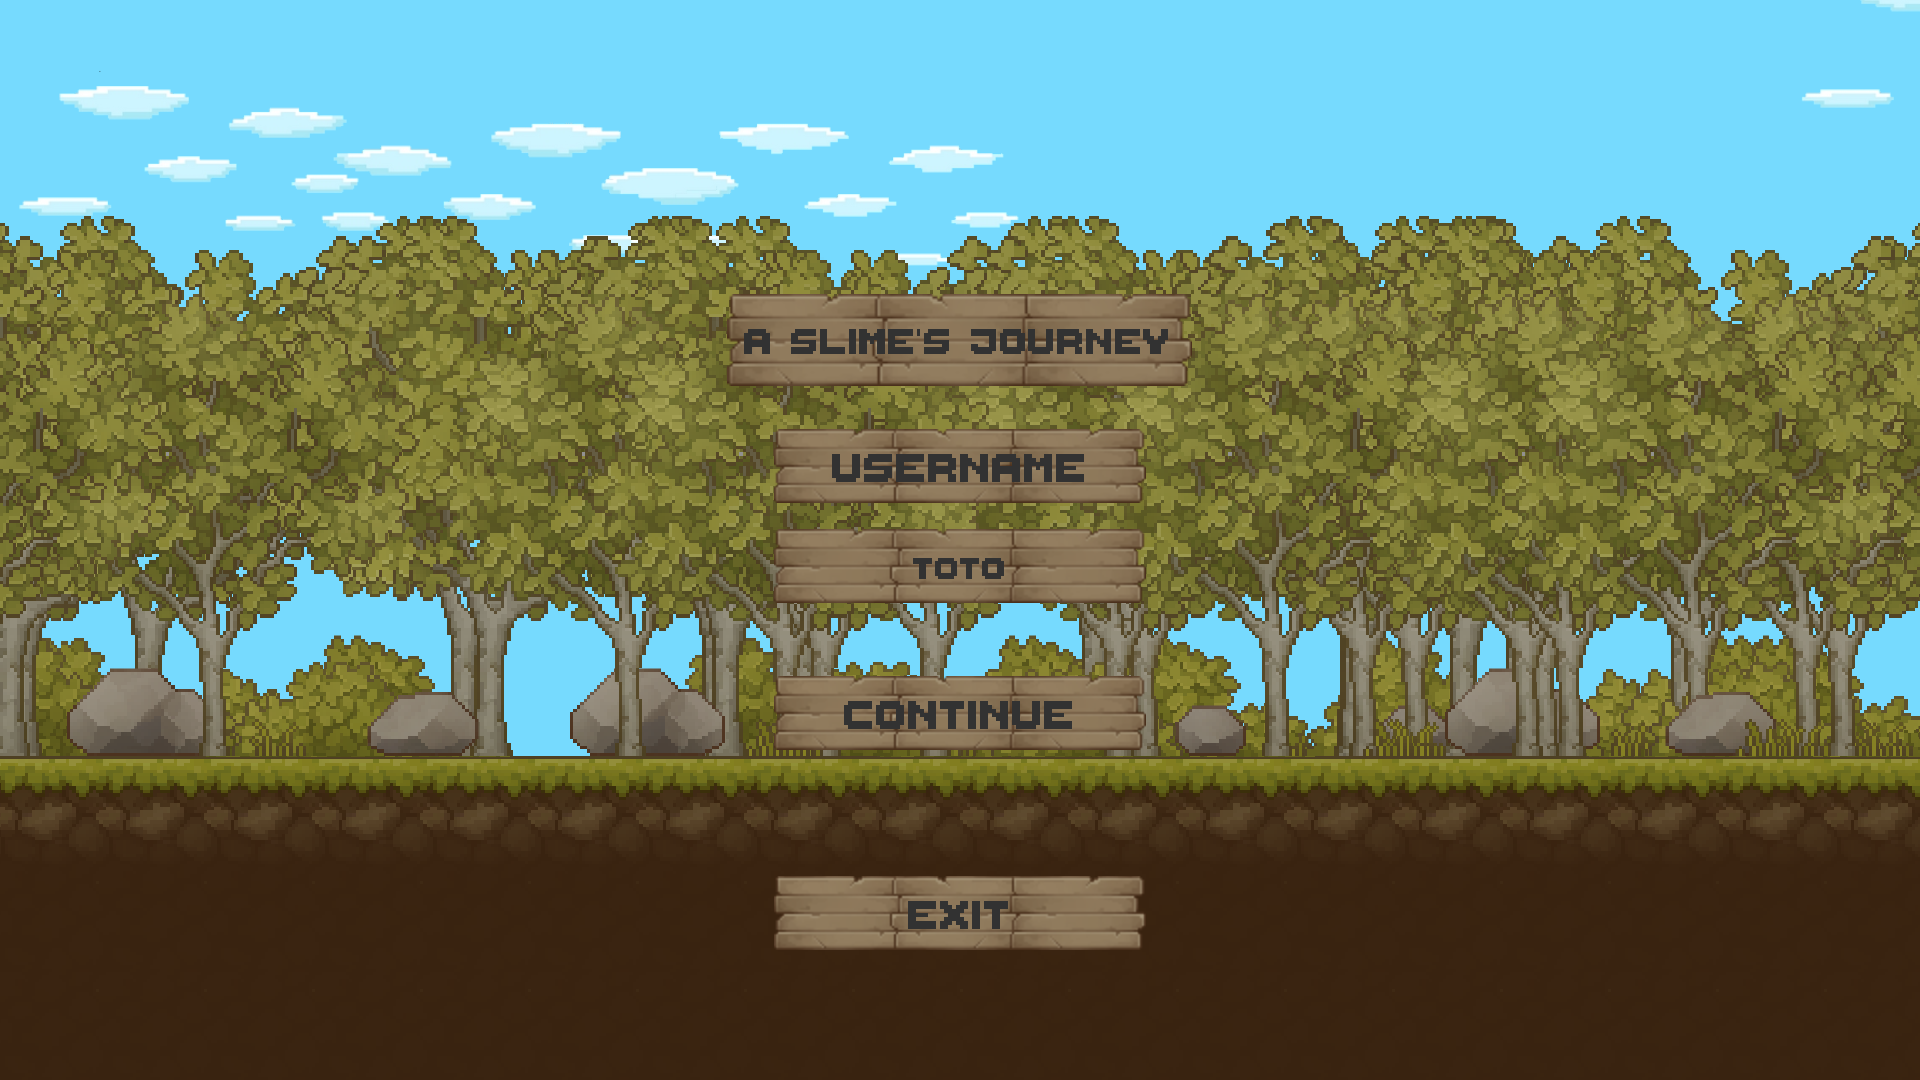
\includegraphics[width=0.49\linewidth]{MMV21.png}
            \end{figure}

            Nous avons alors dessiné la forme du premier niveau qui sera un niveau qui servira de tutoriel au joueur afin qu'il comprenne comment prendre en main le jeu. Après de nombreuses esquisses s'inspirant du design du premier niveau des jeux “Mario”, nous avons fini par réaliser l'ébauche de ce niveau qui par la suite sera implémenté par Alexis dans le jeu.

            De surcroît, le fait d'avoir dû reprendre depuis le départ ce projet nous a aussi permis de corriger plusieurs erreurs qui auraient pu nous créer des bugs dans la suite de la réalisation de ce projet. Nous avons, par exemple, résolu le problème du fait de la synchronisation des caméras afin que chaque joueur ai une caméra différente.
        	
            Nous avons aussi implémenté un système de vie et de mort, empêchant alors le joueur de continuer la partie si celui-ci perds ses 3 vies. Nous avons décidé de faire en sorte que le joueur perde une vie s' il se fait toucher par un ennemi ou encore s' il tombe dans le vide.

            \begin{figure}
                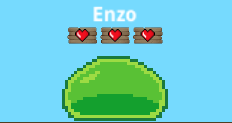
\includegraphics[width=0.49\linewidth]{Slime1.png}\hfill \hfill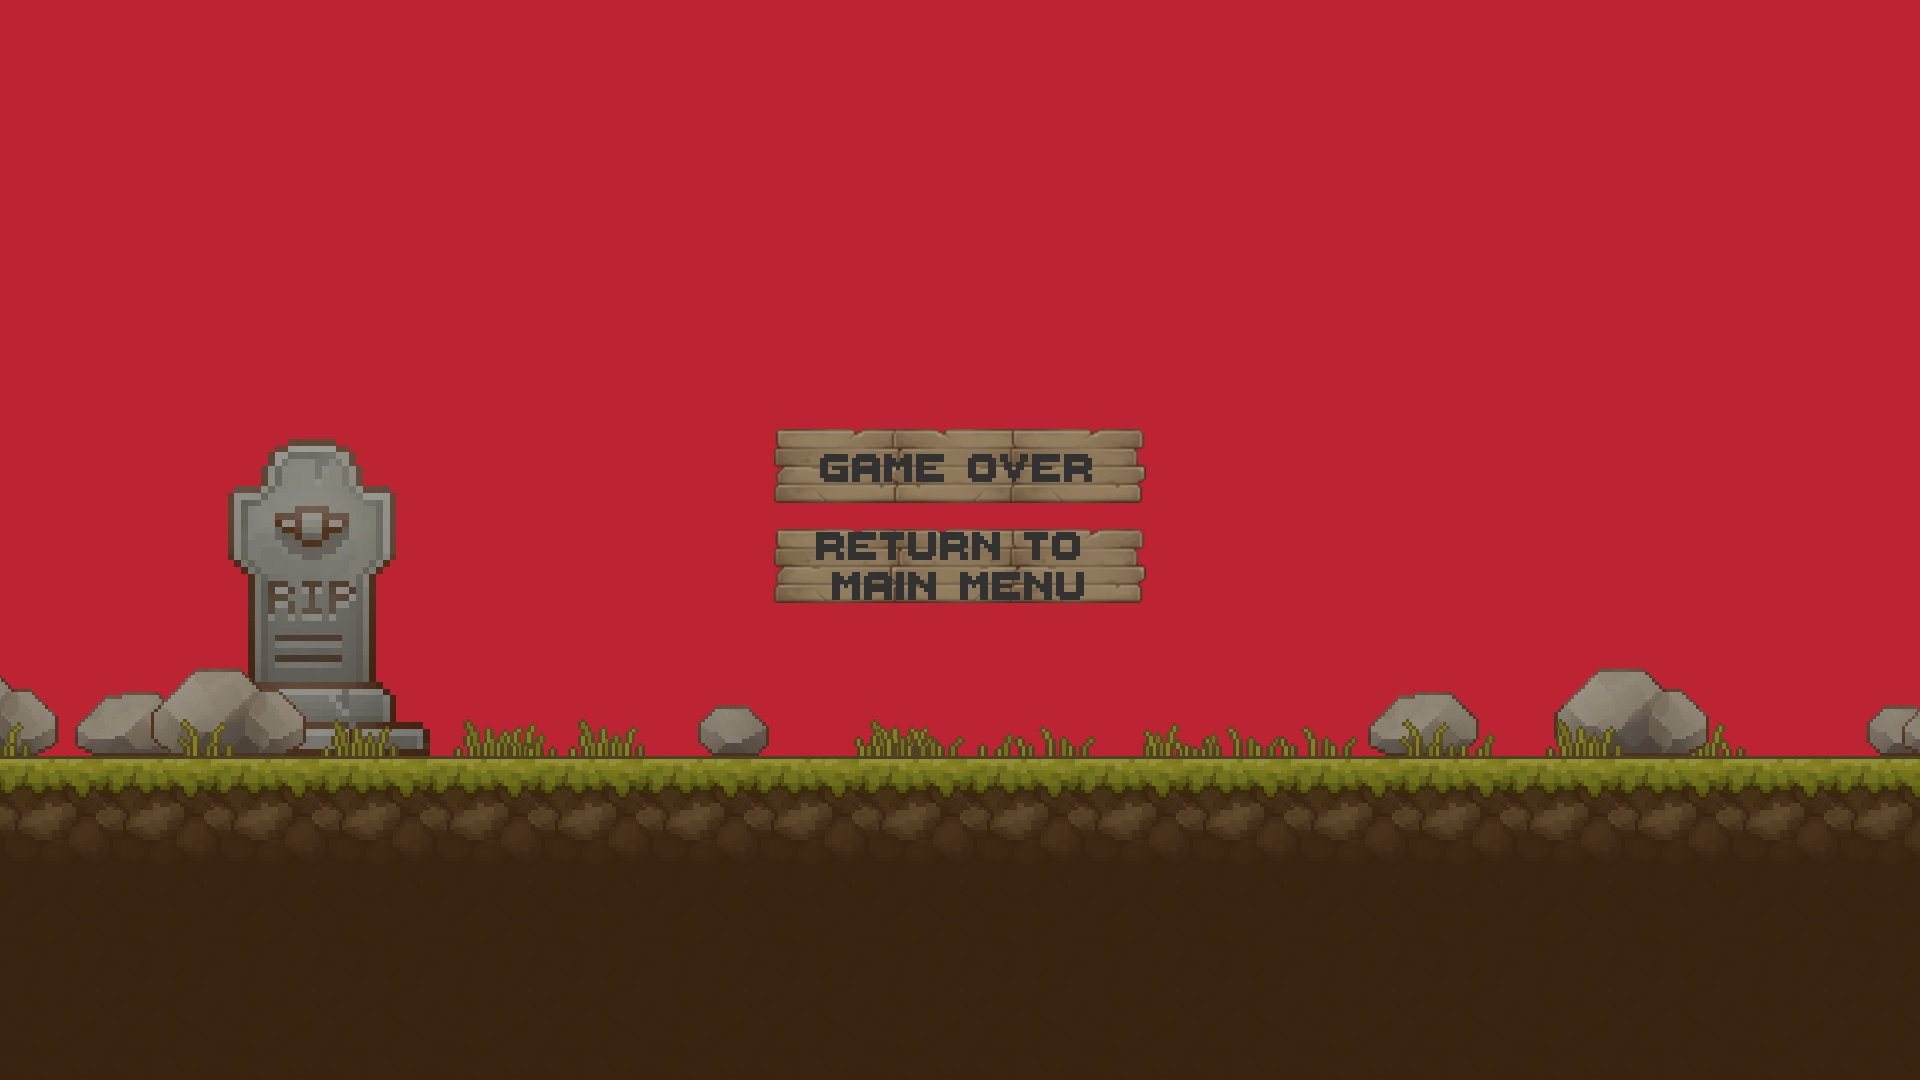
\includegraphics[width=0.49\linewidth]{GameOver.png}
            \end{figure}
        \end{indt}

        \begin{indt}{\subsection{Alexis}}
            Suite à notre première réunion, j'ai réalisé un UML de notre jeu, nous avons immédiatement commencé à implémenter la physique du jeu avec Maxime tels que les déplacements et le saut.

            J'ai aussi implémenté le mode en ligne, le système de rooms et l'instantiation du joueur dans ces dernières , mais des bugs de caméra survenaient et a chaque fois qu'on résolvait un problème un nouveau survenait, donc nous avons décidé de recommencer le projet de zéro pour repartir sur un projet plus propre.

            Suite à ça j'ai implémenté le premier niveau, avec les croquis d'enzo et mis en place les décors, nous avons cherché à faire un premier niveau simple pour que le joueur puisse facilement prendre en main le jeu.

            \begin{center}
                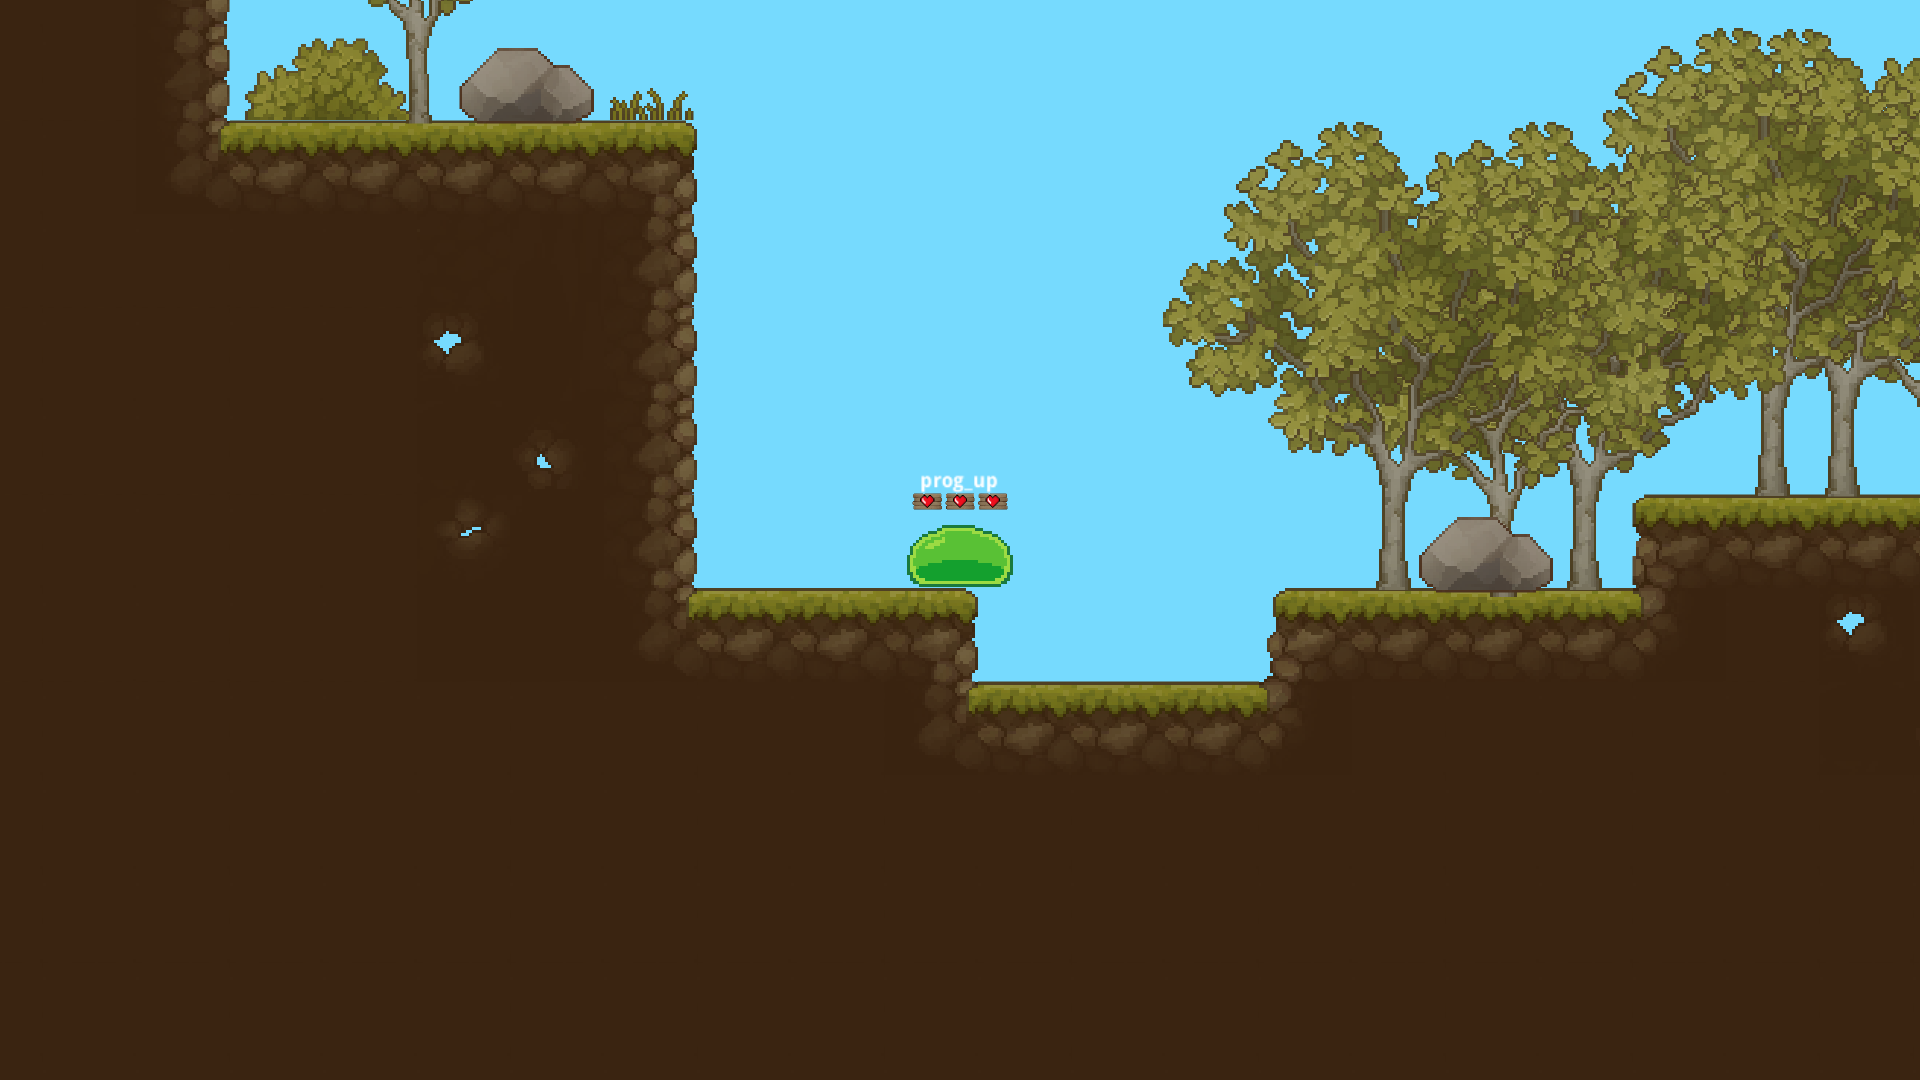
\includegraphics[width=0.8\linewidth]{Lvl1.png}
            \end{center}
        \end{indt}

        \begin{indt}{\subsection{Omid}}
            Tout d'abord, j'ai suivi de nombreux tutoriels afin de mieux comprendre le fonctionnement de Unity et de découvrir la réalisation d'un jeu. J'ai pu découvrir comment utiliser la Tilepalette qui permet de créer nos niveaux en 2D en plaçant un échantillon (de sol par exemple) sur un case et comment fonctionnait les Colliders et Rigidbody (zone de collision, physique du jeu, gravité, …). Après les premières implémentations de Maxime et Alexis sur les mouvements du joueur, j'ai commencé à travailler sur notre premier ennemi: un serpent qui se baladait entre deux points, notre première intelligence artificielle. J'ai donc pu implémenter son animation de déplacement et une des manière que nous avions prévu d'utiliser pour éliminer les ennemis : leur sauter sur la tête. 

            Ensuite, j'ai aidé mes camarades à débugger le saut qui a nécessité de nombreux changements (voir partie sur le saut) et j'ai commencé à chercher d'autres ennemis car le serpent ne correspondait pas vraiment au type d'ennemis que l'on cherchait. Entre temps, on a recommencé le projet à 0, j'ai surtout participé à réimplémenter les mouvements et les ennemis. Cela m'a permis de remplacer le serpent par le sanglier utilisé actuellement. Je lui ai aussi rajouté une animation de mort qui s'active lorsque le joueur lui saute dessus. J'ai ensuite encore modifié le saut afin que le slime soit capable de sauter lorsqu'il est collé à un mur ce qui sera utile pour une prochaine compétence.

            Enfin, j'ai pu rajouter la musique du menu et celle du premier niveau notamment à l'aide des musiques présentes sur le Unity Asset Store.
        \end{indt}

        \begin{indt}{\subsection{Maxime}}
            Tout d'abord, j'ai moi aussi suivis de nombreux tutoriels sur comment utiliser Unity. Ensuite, nous nous sommes tous réunies afin de mettre en place les outils nécessaires afin de pouvoir communiquer entre nous de manière efficace. Cela fait, Alexis et moi avons commencé à implémenter nos  toutes premières fonctions ; les déplacements du joueurs. Suite à cela, Alexis à implémenter la partie multijoueurs, ce qui nous à créer beaucoup de bugs, que nous n'arrivons pas à réparer.

            Afin de pallier cela, nous avons d'un commun accord recommencer de zéro le projet, en gardant uniquement les sprites choisis auparavant afin d'avoir un projet plus propre et plus malléable pour la suite. 
            
            Ensuite, nous avons ré-implémenté le multijoueur Enzo et moi, puis avons fait beaucoup de fonctions de déplacements, toujours avec un saut avec contenant des problèmes. 

            Enfin, je me suis occupé de créer le site internet du projet, qui n'est pour le moment pas complet et n'est qu'un site disponible en local, ne permettant pas encore le téléchargement du jeu et ne comprenant qu'une rapide description du jeu, tout en donnant le style graphique à l'aide d'un fond qui reprend une capture d'écran de notre premier niveau.
        \end{indt}
    \end{indt}
    
    \begin{indt}{\section{Avance / Retard}}
        Au niveau des avances par rapport au planning nous avons pu implémenter un système de mort, ainsi que son écran de fin de partie. En effet, le système de vie et de prendre des dégâts permet véritablement d'ajouter un enjeu au jeu. 

	    Pour ce qui est des retards, on a plutôt respecté le planning hormis pour un point important pour notre jeu: la transformation du slime. En effet, même si notre jeu est actuellement jouable, les transformations du slime permettent véritablement de distinguer “A Slime's Journey” des autres jeux de plateforme. Un petit détail visuel qui n'a pas pu être réalisé est le fait de pouvoir visualiser le château  en arrière-plan depuis le menu principal. Les nombreux problèmes liés au multijoueur ont notamment été responsables d'une perte de temps notable.

	    Finalement, le planning a été plutôt bien respecté car chacun a fait sa part du travail tout en s'entraidant. La communication a été efficace et les différentes réunions se sont très bien déroulées. Cependant, il y a quand même des points sur lesquels on pourrait faire mieux. Tout d'abord, on aurait pu commencer plus tôt à regarder des tutoriels afin de commencer avec quelques connaissances au lieu d'apprendre tout en développant le jeu. On aurait dû aussi recommencer le projet plus tôt que le 3 Mars car on a pu réimplémenter tout ce l'on avait fait auparavant en quelques jours et régler les problèmes de caméra du multijoueur.

    \end{indt}

    \newpage

    \begin{indt}{\section{Rapport des avancées}}
        La prise en mains de Unity 3D à été un peu compliquée au début mais nous nous sommes vite habitué et grâce aux nombreux tutoriels disponibles sur internet, sous la forme de cours ou de vidéo. De plus, l'ensemble des scripts utilisés par ce moteur ont été programmé en C$\#$ avec Visual Studio Code et Rider grâce au Développer Pack du .NET Framework 4.7.1.

        La mise en place du site web fut difficile quant à la mise en place du site internet.

        \begin{indt}{\subsection{Graphismes}}
            Cette section regroupe tout le travail graphique lié au jeu. Tout d'abord, il y a la conception de l'interface du menu principal puis du premier niveau. En effet, grâce à un pack d'assets Unity, nous avons déjà réalisé le premier niveau de A à Z, en se basant sur un plan de celui-ci fait préalablement au croquis. Nous allons également devoir faire de la modélisation graphique des prochains niveaux ainsi que boss, tel qu'il sera prévu, le second niveau sera un village, accessible directement en sortant de la forêt.

            \begin{center}
                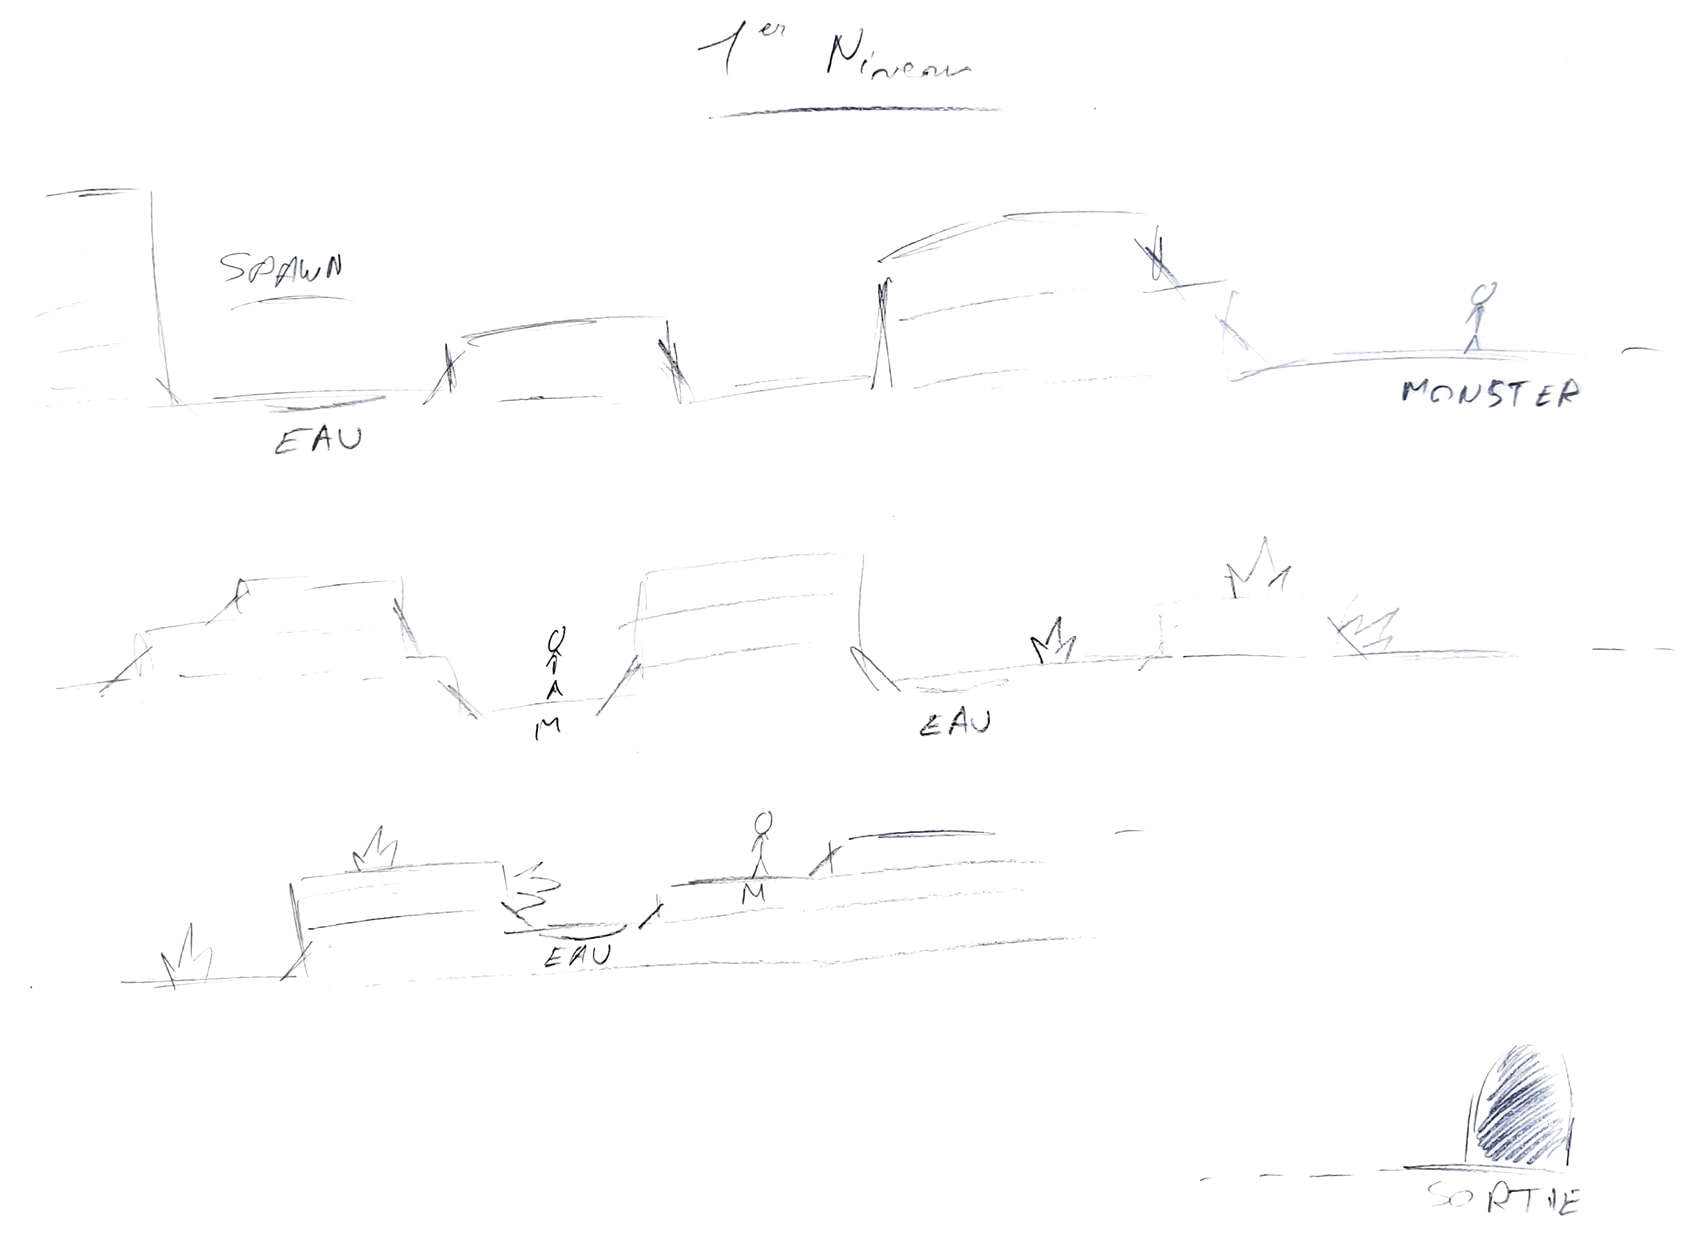
\includegraphics[width=0.5\linewidth]{Croquis.jpg}
            \end{center}

            Concernant le menu principal et le premier niveau, de la conception sur papier à la réalisation sur Unity, il nous à fallu environ un jour de travail cumulée. Le tout fut réalisé sur un même projet Unity synchronisé sur tous les ordinateurs personnels des membres du groupe grâce à Github.

            Premièrement le menu principal fut désigné en vue d'un futur système de sauvegarde à 3 emplacements et de 3 parties en ligne joignable à tout moment dans la limite de 2 joueurs par partie. Il s'est avérée que suite à la réinitialisation du projet, l'objectif de ce menu fut remis en question, ce qui a permit à l'élaboration d'une menu bien mieux construit et aéré, où il est uniquement possible de se connecter à des partie en ligne selon leurs nom, permettant la création d'autant de partie que souhaité, et étant donné qu'aucun système de sauvegarde n'est encore implémenté. Ainsi, les seuls boutons que l'on a gardés permettent de se déplacer entre les menus, permettant de lancer une partie, la quitter, relancer une autre partie et quitter le jeu.

            \begin{figure}
                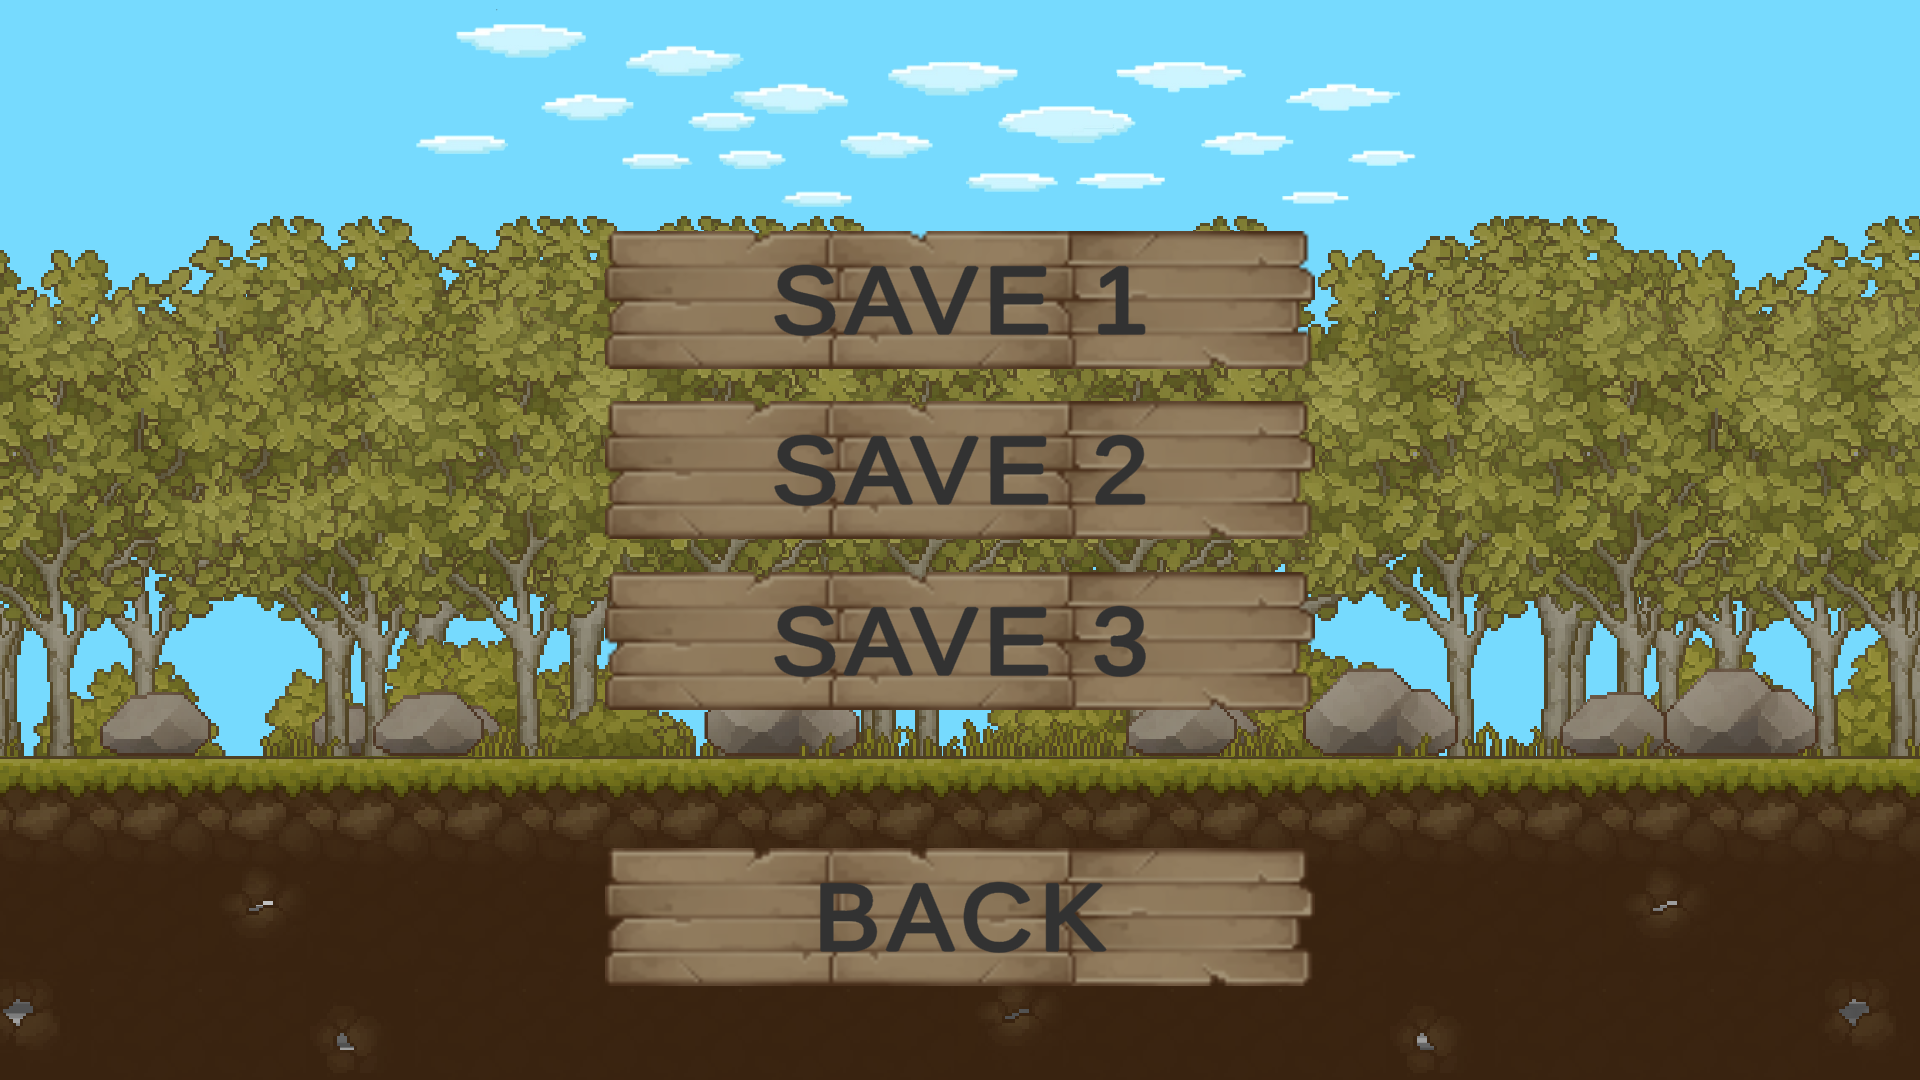
\includegraphics[width=0.49\linewidth]{MMV12.png}\hfill \hfill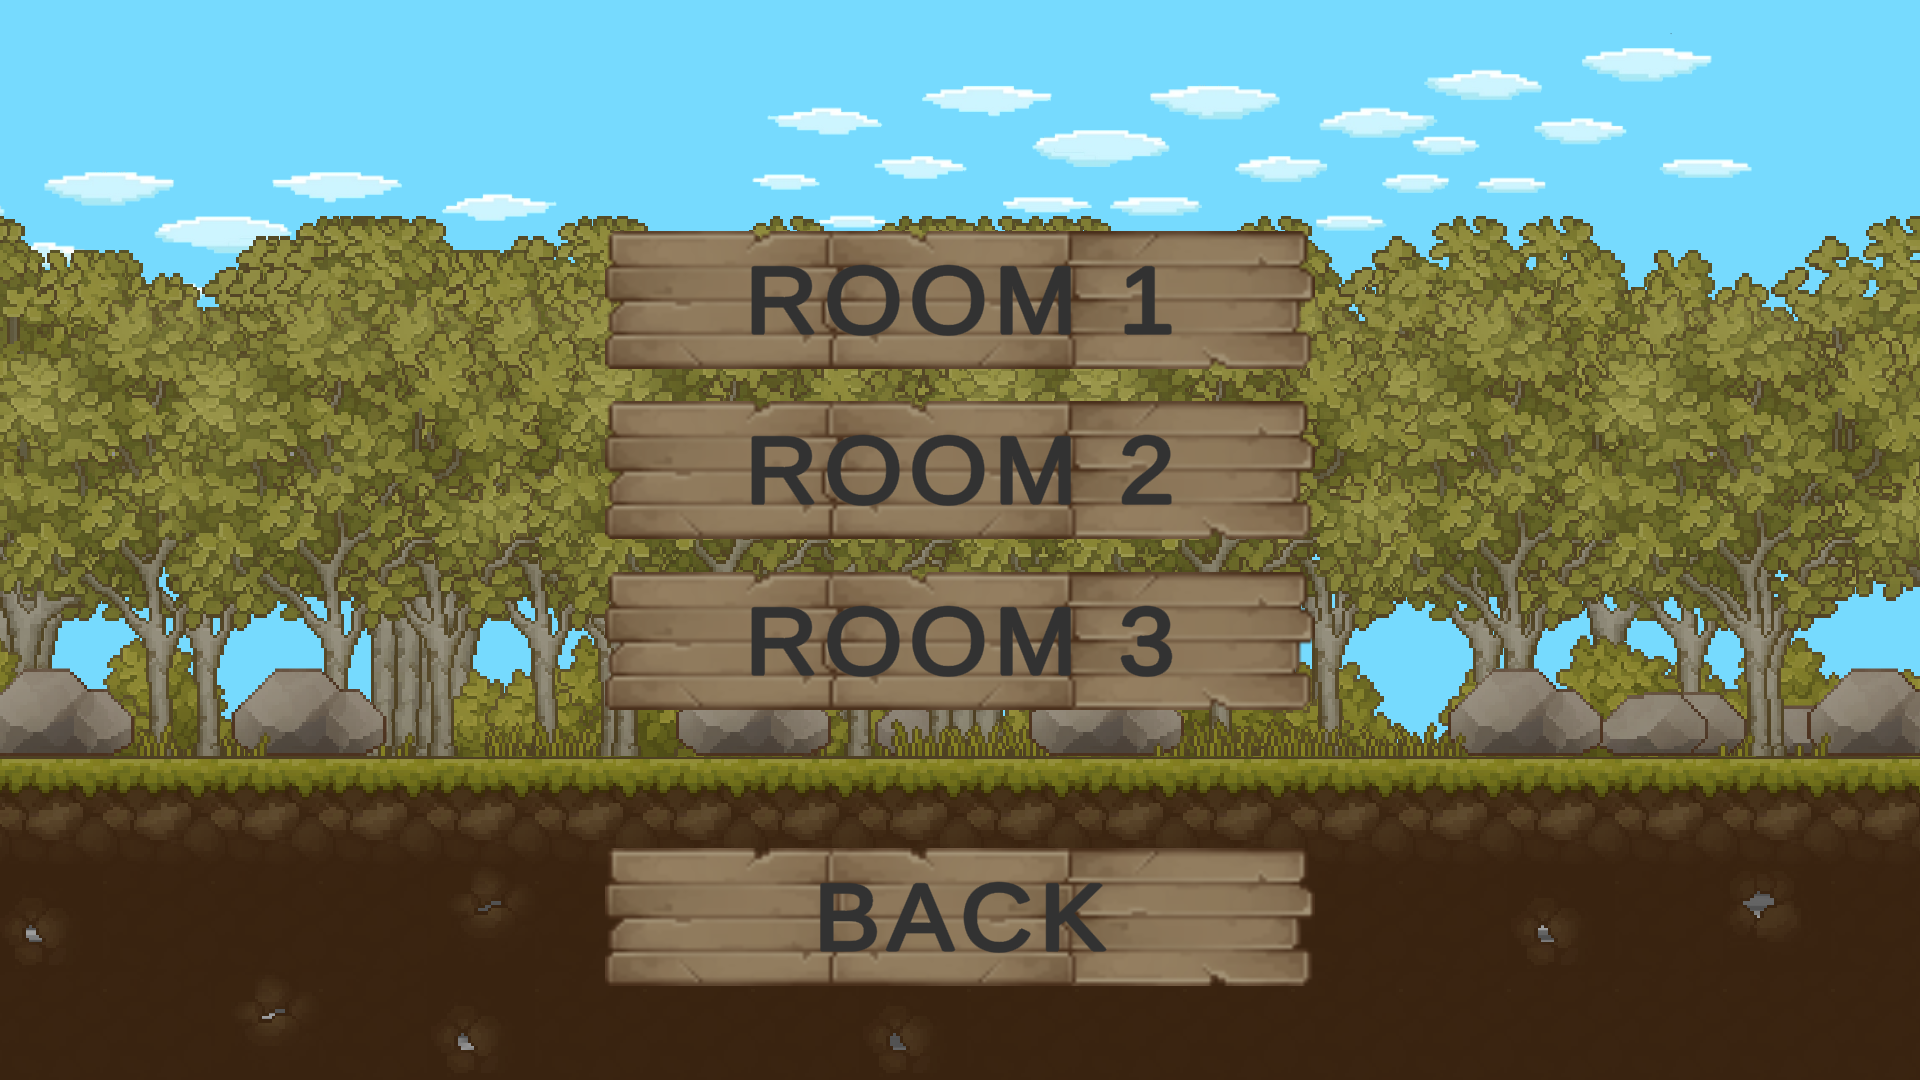
\includegraphics[width=0.49\linewidth]{MMV13.png}
                %\caption{Avant} \label{fig:twographs}
            \end{figure}

            \begin{figure}
                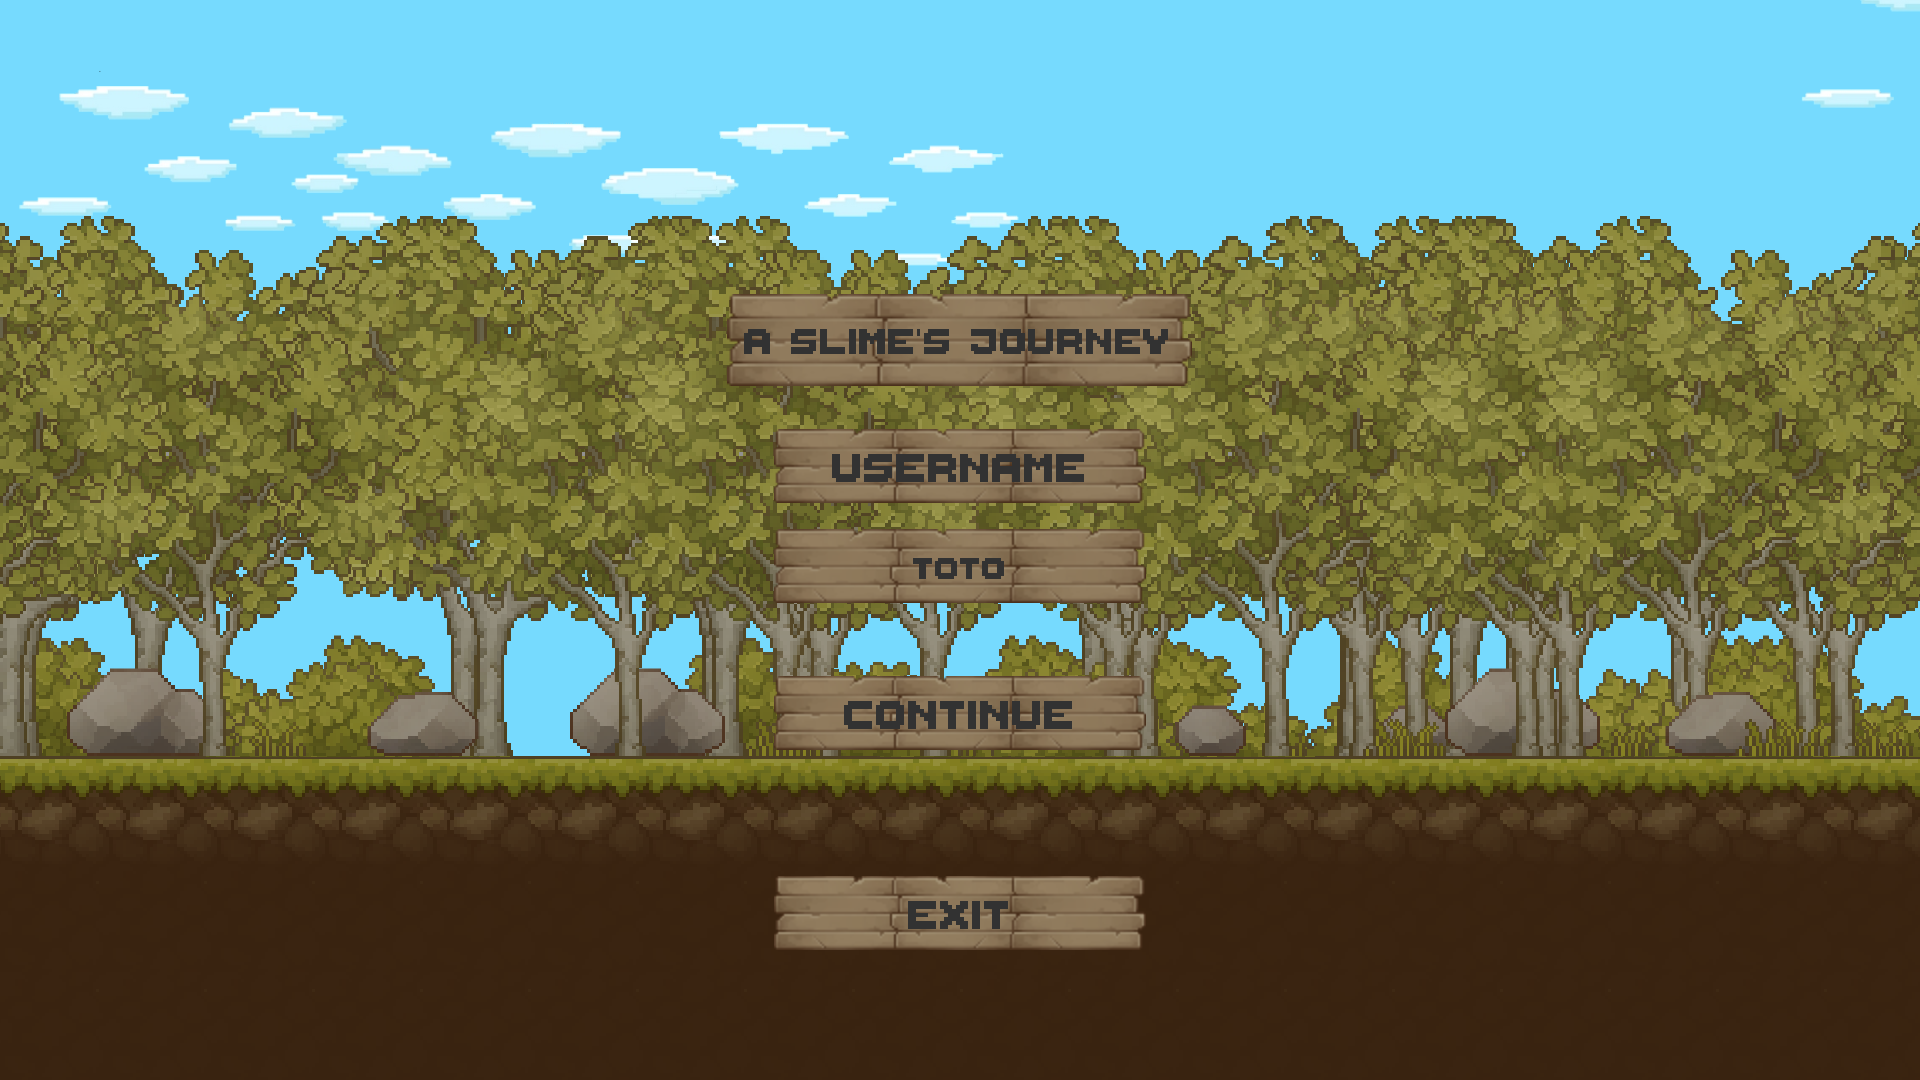
\includegraphics[width=0.49\linewidth]{MMV22.png}\hfill \hfill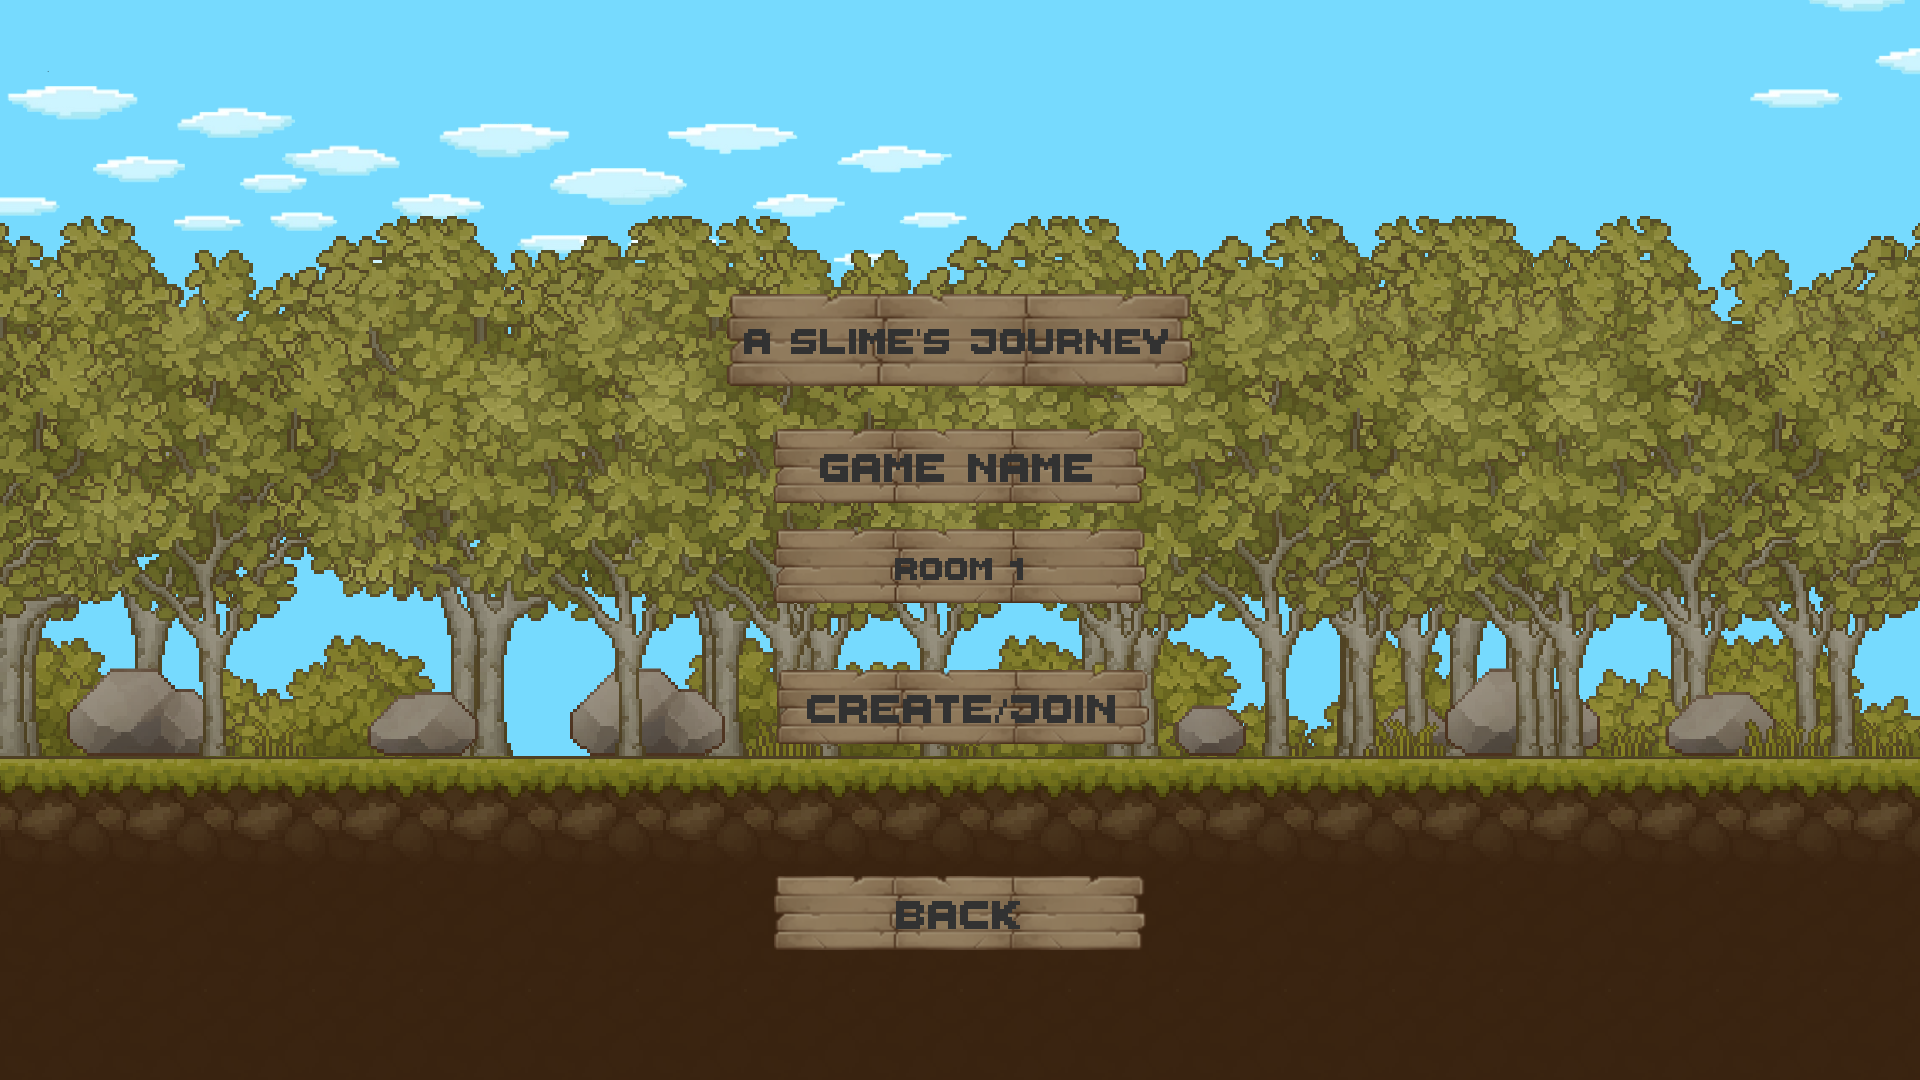
\includegraphics[width=0.49\linewidth]{MMV23.png}
                %\caption{Après} \label{fig:twographs}
            \end{figure}

            De manière générale, pour conserver une ambiance médiévale tout au long du jeu, nous avons importé un paquet unity nommé “Pixel Art Platformer - Village Props”. Qui nous permet de facilement créer des niveaux grâce aux plateformes implémentés avec collisions et à l'ensemble des décors fournit. C'est d'ailleurs avec le panneau de ce paquet qu'à l'aide du logiciel de retouche d'image Photofiltre, qu'il fut transfomé en la texture utilisé par tout les boutons du jeu, ainsi qu'avec un filtre noir et blanc, sert de texture pour un bouton sélectionné. 

            Le Slime quant à lui, est issu du paquet Unity “Slime Enemy - Pixel Art”, de nombreuses animations viennent faciliter son implémentation. Cependant, il sera nécessaire de créer nous même d'autres formes et animations pour les futures transformations.
        \end{indt}

        \begin{indt}{\subsection{Les Logos}}
            Afin de pouvoir faire connaître notre jeu ainsi que notre entreprise, il nous fallait des logos pour nous différencier des autres. Étant tous intéressés par les mathématiques nous nous sommes tous mis d'accord sur le nombre d'euler, c'est pour cela que notre entreprise s'appelle ARCLN et que notre logo représente une courbe exponentielle.
        
            \begin{center}[h!]
                
\includegraphics[width=0.5\linewidth]{Logo2.png}
            \end{center}

            Pour notre logo de jeu, nous avons choisi de représenter au mieux l'esprit de notre jeu en créant un logo à la fois rustique et simple, un logo parfait pour un jeu se déroulant dans un univers médiéval.
        \end{indt}

        \begin{indt}{\subsection{Site internet}}
            Le site internet à été créé par nous même, en utilisant le HTML, et contient un CSS afin de pouvoir mieux gérer la mise en page du site. Tout d'abord, la création du site en lui-même, en passant par l'application bloc-note afin de savoir ce qui était important de mettre sur le site internet. Ensuite, viennent les idées, tel que la mise en arrière plan d'une capture d'écran de notre premier niveau, indiquant le titre du jeu affiché sur une pancarte du menu du jeu, afin de montrer clairement la direction artistique du jeu. L'affichage de l'arrière-plan fut problématique, en effet, l'image n'était pas assez grande, par conséquent, les commandes habituelles afin de faire un arrière-plan qui couvre toute la page était impossible. Après plusieurs essais non concluants, la décision d'agrandir la partie intéressante de l'image à été prise, afin de contourner notre problème.
        \end{indt}

        \begin{indt}{\subsection{Multijoueur}}
            C'est la première chose qui a été implémentée dans le projet Unity grâce à Photon, une extension de Unity permettant de créer un jeu vidéo en ligne avec une API complète et l'utilisation gratuite de leurs serveurs pour héberger les parties. Cela fut possible avec le tutoriel disponible sur leur site et c'est pourquoi, lors de notre première version, on ne pouvait que rejoindre des parties générées aléatoirement. Mais après la remise à zéro du projet, comme on avait tous pris connaissance de l'API de Photon, on a pu, de manière bien plus complète, réimplémenter un système de multijoueur proprement. Cette implémentation nous a permis d'interfacer le multijoueur de manière à pouvoir créer et rejoindre des parties en fonction de leur nom.

            Comme voulut dans le cahier des charges, le multijoueur permet de jouer en coopération au sein d'une même partie. Dont l'unique but est de faciliter l'avancée du joueur sans en augmenter la difficulté de la partie. C'est ainsi que l'ajout d'un joueur se fait avec l'apparition d'un message en bas à gauche de l'écran en vert et à contrario si un des deux joueurs se déconnecte, un nouveau message apparaît en rouge. De plus, chaque joueur à son pseudo d'afficher au-dessus de lui ainsi que les vies qu'il possède, sachant qu'il en a 3 au début de chaque partie.

            On a implémenté le réseau dans le jeu avec un système de “rooms” à créer ou à rejoindre avec des noms de parties, les joueurs entrant les même noms de rooms se retrouveront donc dans la même room, de plus si un des deux joueurs meurt, ce joueur quittera la room, le joueur peut aussi quitter la room en utilisant le menu en pleine partie avec le bouton echap. L'instantiation des rooms se fait par le menu principal avec Photon. 
        \end{indt}

        \begin{indt}{\subsection{Caméra}}
            La caméra fut un des éléments les plus embêtants à gérer et est d'ailleurs une des principales raisons pour lesquelles on a décidé de recommencer le projet le 3 Mars. 

            Au début, nous avions fait en sorte que la caméra qui suit le joueur soit la caméra principale du jeu. Nous avions fait un script qui fait déplacer la caméra avec les déplacements du joueur. Cependant, même si cela marchait parfaitement en mode solo, en multijoueur la caméra principale n'arrivait pas à suivre les deux joueurs quand les deux bougeaient en même temps. Nous avons donc ensuite créé une caméra liée au joueur dans le dossier Ressources de Photon, créée en dehors de la scène du niveau. Cela permet de faire en sorte que chaque joueur ait sa propre caméra lorsque l'on lance le jeu. Théoriquement, cela aurait dû marcher parfaitement. Tout d'abord, la caméra suivait bien le joueur mais ne montrait rien. On a pu régler ce problème en reculant la caméra sur l'axe z. Ensuite, bien qu'en solo cela marche très bien, en multijoueur, les caméras des deux joueurs s'inversaient. En effet, le joueur déjà présent sur le niveau prenait la caméra du joueur qui avait rejoint et ce dernier prenait la caméra du joueur déjà présent.

            Ainsi, c'est à ce moment-là que nous avons décidé de recommencer le projet afin d'avoir un projet plus propre et de recommencer avec des bases solides. Lors de la première version, nous avions eu de nombreux problèmes avec la caméra, en effet, lors d'une partie en solitaire, le joueur avait bien la caméra réglée sur lui, qui la suivait correctement. Les problèmes arrivent lors d'une partie en multijoueurs, en effet, lorsque le premier joueur se connecte, il a sa propre caméra, mais, lorsqu'un second joueur se connecte, la caméra du joueur 1 va sur le joueur 2 et la caméra du joueur 2 va sur le joueur 1. Cela est dû au fait que la nouvelle instance de caméra essaye de se fixer sur le dernier joueur créer, ou alors de se fixer sur la première autre instance de joueur qu'il trouve sans caméra.

            Suite à notre incapacité à résoudre ce bug, nous avons décidé de recommencer le projet en partant de rien.

            C'est à partir de ce constat que nous avons ré-implémenté le multijoueur afin de régler ce bug majeur, et d'autres bugs mineurs liés au multijoueur. Cela étant fait, nous avons dû faire face à un autre bug de caméra, le dernier joueur à rejoindre avait la bonne caméra, nous avions juste oublié de désactiver la caméra si elle n'appartient pas au bon joueur lors de l'instanciation du nouveau joueur.

        \end{indt}

        \begin{indt}{\subsection{Intelligence Artificielle}}
            Nous avons décidé d'implémenter l'IA via les différents ennemis. En effet, chaque ennemi a un comportement différent selon ses capacités et/ou ce que fait le joueur. Pour l'instant, un seul ennemi a été implémenté: le sanglier. Ce dernier se déplace entre deux points définis au préalable. En effet, à chaque instant le programme vérifie la position du sanglier par rapport à un des deux points qui est ciblé et tant qu'il n'a pas atteint ce point  il avance vers ce point avec une vitesse prédéfinie. Lorsqu'il atteint le point visé, il prend le second point pour cible et commence à avancer vers lui. 

            Par rapport au joueur, il ne change de comportement que lorsque ce dernier lui saute dessus, c'est-à-dire lorsque la zone de contact du slime et une zone au-dessus du sanglier entrent en contact. Le sanglier va alors lancer son animation de mort et s'autodétruire 0,5 seconde après le contact. De plus, le joueur sera propulsé dans les airs grâce à un attribut de PhysicMaterial 2D avec une propriété de rebondissement. Cette technique de patrouille entre deux points  peut aussi être adaptée afin de faire en sorte que l'ennemi poursuit le joueur tout simplement en mettant le point visé sur le joueur ce qui pourra être utile pour de prochains ennemis. 

            Une autre technique qui a été envisagée pour faire patrouiller l'ennemi est de le faire avancer jusqu'à ce qu'il se cogne dans un objet différent du joueur (mur, objet solide, …), le faisant repartir dans l'autre sens. L'inconvénient avec cette technique c'est que si il n'y a une zone de vide l'ennemi ne va pas s'arrêter et tomber dans le vide, contrairement à la patrouille actuelle où l'ennemi ne dépasse jamais le point cible.

        \end{indt}

        \begin{indt}{\subsection{Mouvements et Saut}}
            Au début, nous avions choisis de se déplacer avec les flèches directionnelles, cependant cela n'était pas très pratique pour le joueur qui devait utiliser ses deux mains juste pour se déplacer et sauter (le saut se faisant sur la touche espace). Nous avons pour l'instant décidé de permettre aux joueurs d'utiliser soit les flèches directionnelles soit la touche A (pour aller à gauche) et la touche D (pour aller à droite). Cependant nous comptons faire en sorte que toutes les touches soient personnalisables par le joueur lorsque nous aurons implémenter toutes les techniques (attaques, inventaires, …).

            Pour déplacer le joueur, nous ajoutons à la position du joueur sa vitesse multipliée par un vecteur dirigeant le mouvement (sens vers la gauche ou vers la droite).

            Le saut quant à lui a été un peu plus complexe à implémenter. Au début nous avons créé deux points : un en bas à gauche du slime et un bas à droite du slime. Ces deux points été utilisés dans la fonction Physics2D.OverlapArea qui crée une zone entre les deux points d'une largeur définie. Cela permettait de vérifier si le slime touchait le sol et donc avait le droit de faire un saut s'il appuie sur la touche espace. 

            Cependant, le saut ne se faisait pas tout le temps. Pour régler ce problème nous avons séparé en deux conditions distinctes : la vérification de l'entrée de la touche espace et la vérification que le slime est bien au sol. 

            Ensuite nous avons modifié la manière avec laquelle on vérifiait que le slime était au sol. Au lieu d'avoir deux points distincts, on en a gardé qu'un seul que l'on a positionné au centre du slime. Nous avons alors utilisé la fonction Physics2D.OverlapCircle qui crée un cercle de rayon de longueur prédéfinis autour du point et qui vérifie si ce cercle est en collision avec un objet avec un layer (couche associée à l'objet) de type Par défaut. Si c'est le cas alors le joueur est soit au sol soit sur un mur car nous voulions que le slime soit capable de sauter lorsqu'il est collé au mur. On a aussi dû rajouter un layer de type Player au joueur afin que le joueur ne puisse pas sauter à l'infini. 

            L'animation du saut du slime n'a pas encore été implémentée mais sera faite très prochainement. Le saut à encore quelques problèmes, en effet, il permet au slime de rester accroché aux murs, ce qui n'est pas souhaitable comme capacité de base du slime.

        \end{indt}

        \begin{indt}{\subsection{Musique et Son}}
            Nous cherchions des musiques qui entrent dans l'univers de notre jeu. Ainsi, après de nombreuses recherches et tests sur audacity nous avons trouvé un asset de musiques qui correspondait parfaitement à l'ambiance que l'on voulait donner au jeu. En effet, en plus de coller à l'ambiance médiévale, ces musiques correspondent bien au premier niveau où l'atmosphère est plus posée et joyeuse permettant ainsi aux joueurs de mieux s'intégrer dans l'univers de “A Slime's Journey”.

            Nous avons donc utilisé quelques musiques de l'asset Fantasy RPG adventure disponible sur le Unity Asset Store. Nous utilisons deux musiques différentes : une pour le menu et une pour le premier niveau. Pour chaque scène nous avons ajouté un élément vide avec un attribut Audio Source qui permet de jouer la musique. Les effets sonores n'ont quant à eux pas encore été implémentés mais le principe reste le même qu'avec les musiques en fond, il suffit juste de les activés aux moments opportuns. 

        \end{indt}

        \begin{indt}{\subsection{Gameplay}}
            Dans “A Slime's Journey”, vous allez jouer un slime dans un monde médiéval. Le jeu est en 2D. Pour le premier niveau, le joueur se retrouve dans une plaine ensoleillée et accueillante encore loin du château qui est l'objectif final du dernier niveau. Comme tout jeu de plateformes, le but du jeu est d'atteindre la fin du niveau  en esquivant les nombreux pièges et ennemis afin de poursuivre l'aventure. Pour l'instant, le joueur doit faire face à un seul type d'ennemi, le sanglier, qu'il peut éliminer en lui sautant dessus. Cependant, s'il se fait toucher de face par le sanglier qui court vers lui, le joueur perd une de ses trois vies. Si il perd ses trois vies ou si il tombe dans le vide, le joueur perd la partie et l'écran de fin de partie s'affiche invitant le joueur à retourner au menu. 

            Pour l'instant, il n'y a pas de fin de niveau à proprement parler, cela sera implémenté lorsque d'autres niveaux sont disponibles afin de permettre aux joueurs d'accéder au prochain niveau après avoir fini le premier niveau. Bien évidemment, d'autres fonctionnalités seront implémentés prochainement (voir Projets futurs) tel que les transformations du slime afin d'avoir un gameplay plus dynamique et surtout unique permettant aux joueurs de s'amuser tout en se mettant au défi.

        \end{indt}

        \begin{indt}{\subsection{Bugs et problèmes à régler}}
            Tout d'abord, au niveau du multijoueur, un bug apparaît lorsqu'un joueur rejoint une partie créée alors que le sanglier a déjà été tué par le joueur déjà présent. En effet, le joueur qui a rejoint voit le sanglier sur son jeu et peut se faire tuer par ce dernier tandis que pour le joueur déjà présent  le sanglier n'existe pas. De plus, le multijoueur est la plupart du temps pas très fluide notamment à cause de Photon.

            Au niveau des graphismes, les arbres superposées changent parfois d'ordre lorsque le joueur bouge créant un effet visuel un peu étrange. Par exemple, un arbre posé en arrière plan va venir au premier plan et celui au premier plan va aller à l'arrière-plan. Un autre bug visuel est le fait que parfois il y a des minuscules espaces dans le sol qui laissent entrevoir le fond bleu de la map. Il existe aussi un bug de collision avec les murs, permettant de “s'accrocher” au mur contre notre gré.

        \end{indt}

        \begin{indt}{\subsection{Communication}}
            Pour cette première soutenance, nous n'estimons pas avoir un jeu assez abouti pour commencer à en faire la communication, c'est la raison pour laquelle il n'existe pas encore de page dédiée au jeu sur les réseaux sociaux. Ces pages devraient être créées sous peu, puisque le premier niveau est implémenté, et qu'il est presque sans bug à l'heure actuelle. Le jeu sera présent sur différentes plateformes tel que Youtube, Instagram ou encore Discord. Nous possédons cependant un site qui présente les premier graphismes et aussi le but du jeu, et un compte instagram.
        
            \begin{center}
                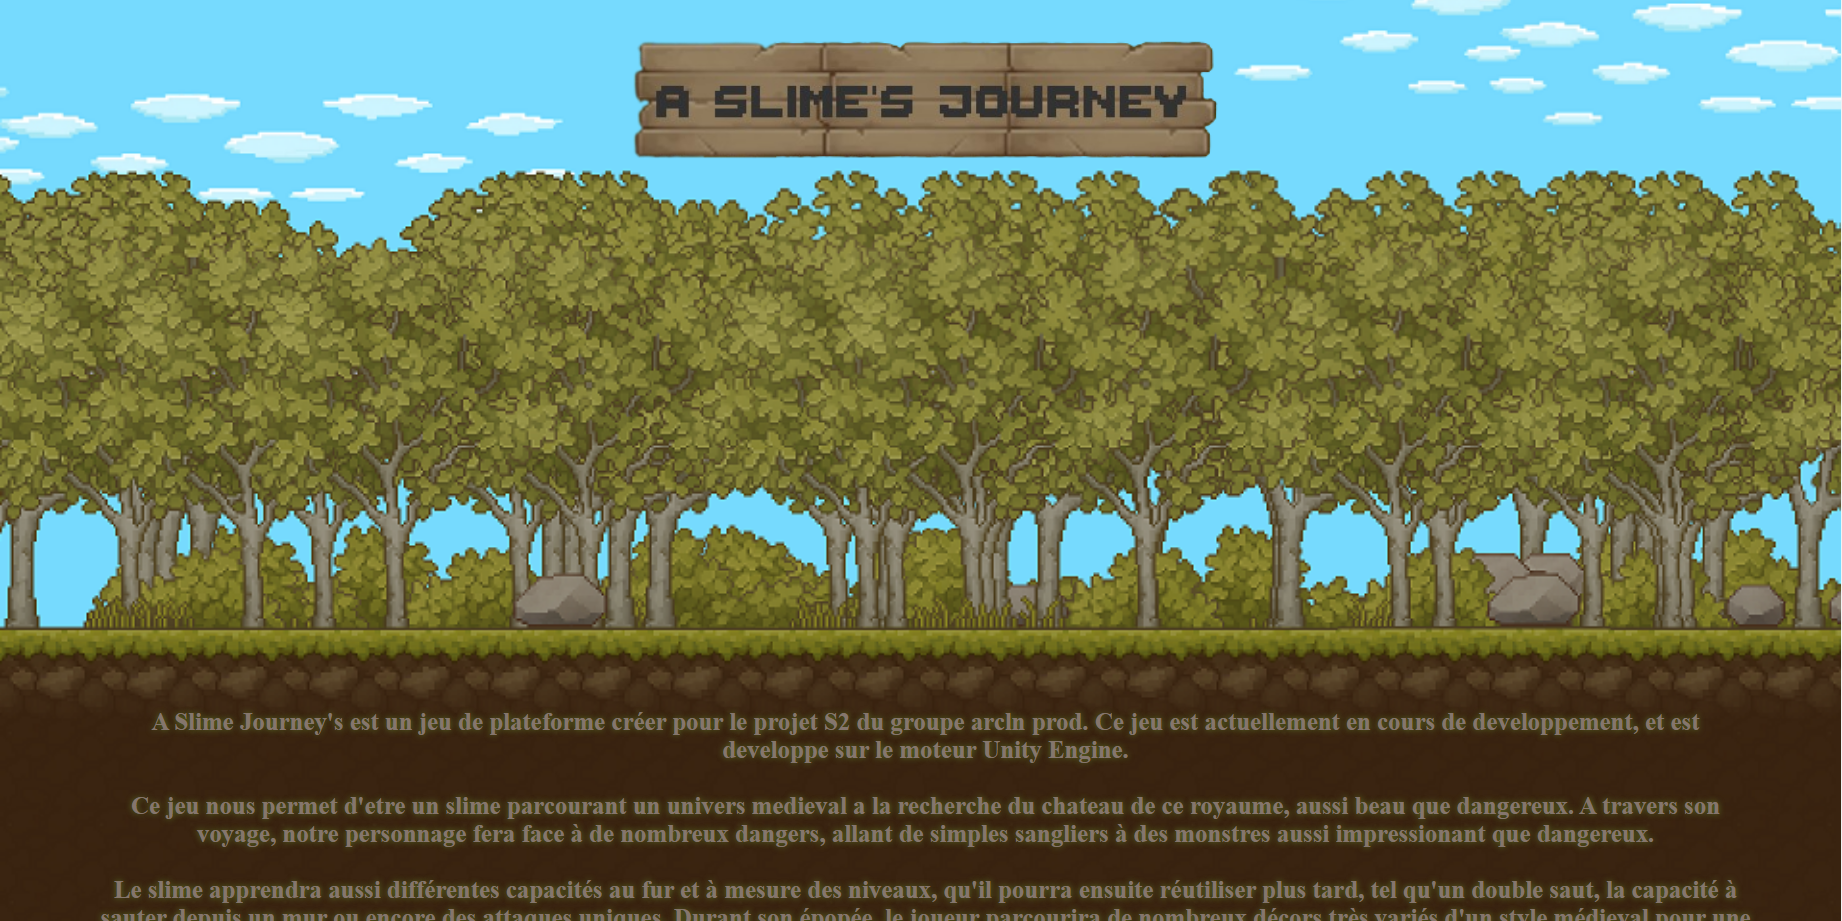
\includegraphics[width=0.8\linewidth]{Site.png}
            \end{center}
        \end{indt}

        \begin{indt}{\subsection{Répartition des tâches}}
            Pour une répartition des tâches efficace et équilibrée, nous avons fait le choix de créer une liste des tâches, celle-ci nous est disponible sous la forme d'un projet sur notre page Github du projet. Ainsi, nous pouvons organiser à l'aide de quatre catégories.
        
            \begin{center}
                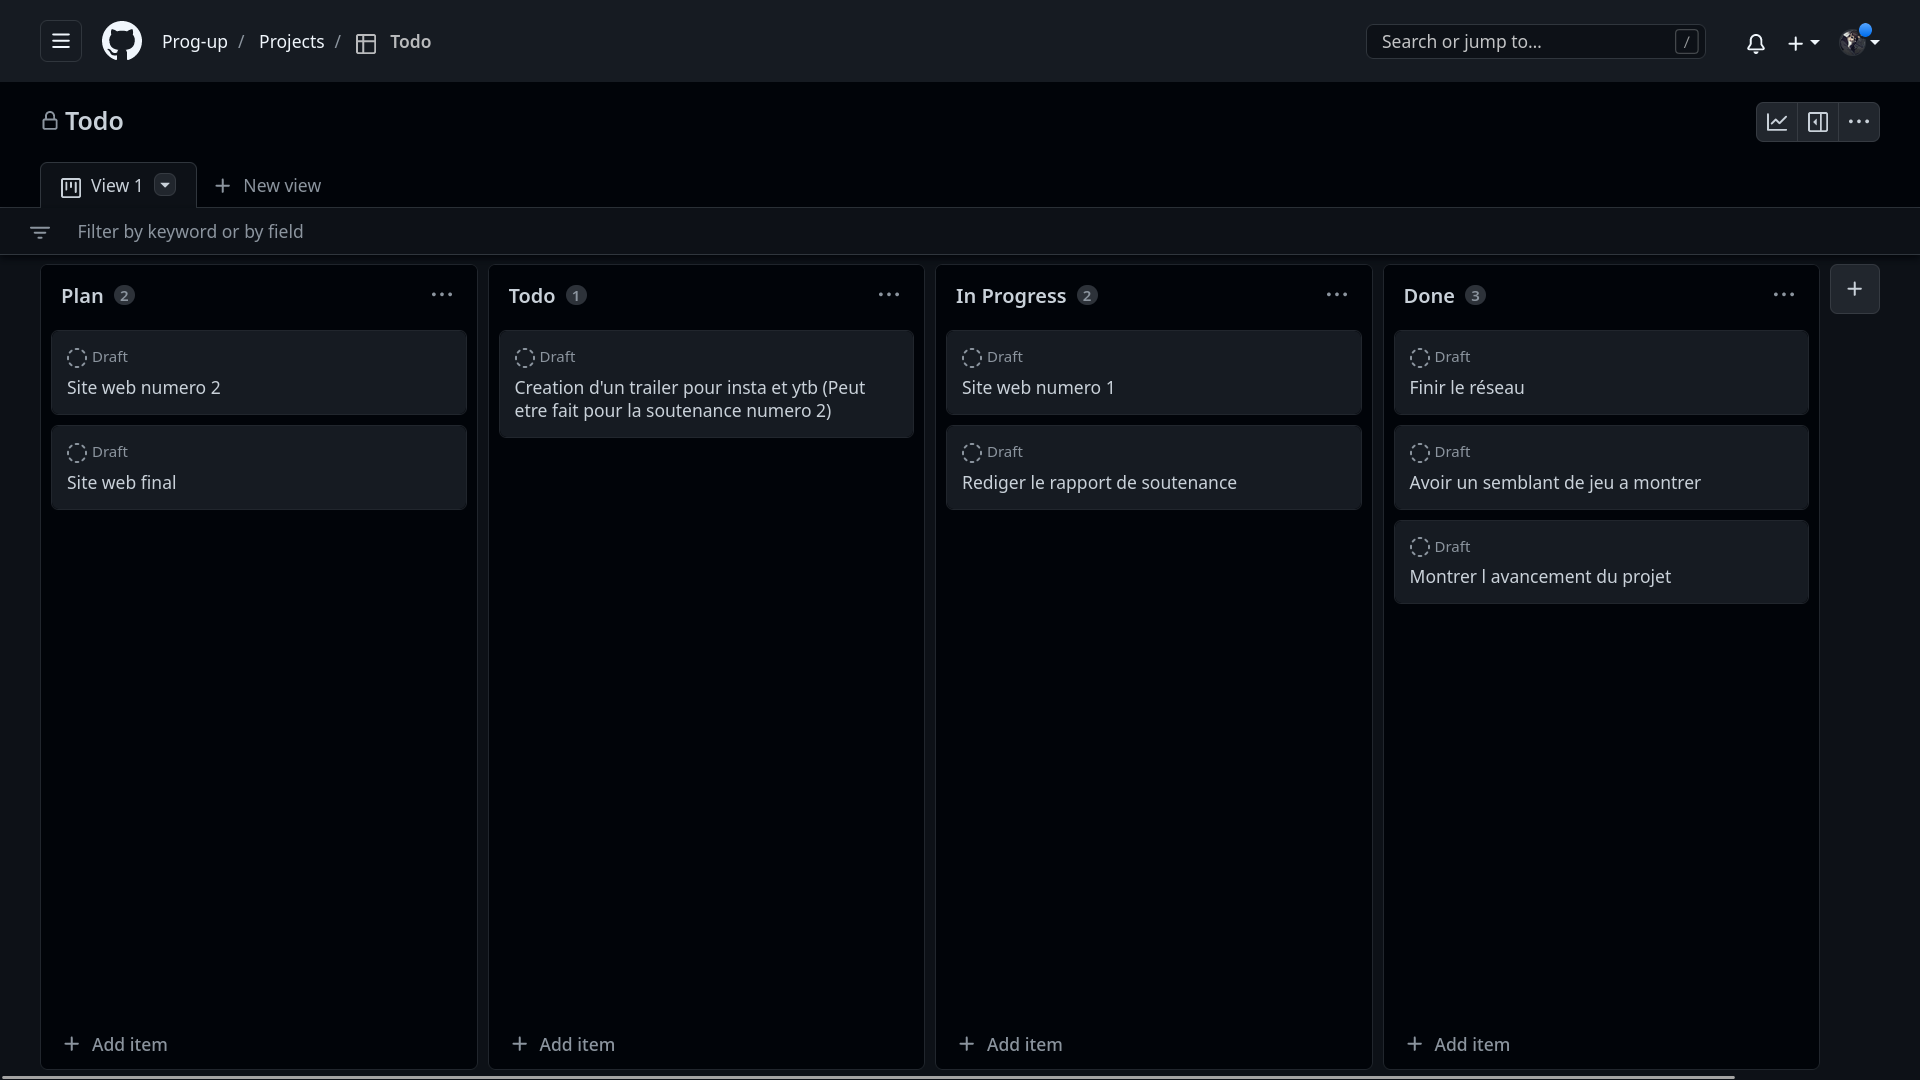
\includegraphics[width=0.8\linewidth]{EDT.png}
            \end{center}

            En plus des tâches disponibles sur Github, le cahier des charges comprend aussi une section dessus, disponible ci-dessous. C'est pourquoi, celle-ci restent nos directives principales, que nous suivons en priorité, malgré que certaines d'entre elles n'ont pas réussi à être implémentés dans les temps tel qu'une transformation du joueur.
        \end{indt}

        \begin{indt}{\subsection{Planning}}
            \begin{center}
                \begin{tabular}{|c|l|l|l|}
                    \hline
                    & Première Soutenance & Deuxième soutenance & Troisième soutenance
                    \\
                    \hline
                    Développement 
                    & \begin{tabular}{l}
                        $\bullet$ 1 niveau 
                        \\ 
                        $\bullet$ Interactions basiques 
                        \\ 
                        $\bullet$ 1 transformation
                    \end{tabular}
                    & \begin{tabular}{l}
                        $\bullet$ Second niveau
                        \\ 
                        $\bullet$ Nouvelles formes
                        \\ 
                        $\bullet$ 1 boss
                    \end{tabular}
                    & \begin{tabular}{l}
                        $\bullet$ Ajout derniers niveaux
                        \\ 
                        $\bullet$ Mode boss rush
                    \end{tabular}
                    \\
                    \hline
                    Communication 
                    & \begin{tabular}{l}
                        $\bullet$ Site Web
                    \end{tabular}
                    & \begin{tabular}{l}
                        $\bullet$ Réseaux sociaux
                    \end{tabular}
                    & \begin{tabular}{l}
                        $\bullet$ Sortie officielle du jeu
                    \end{tabular}
                    \\
                    \hline
                    Design 
                    & \begin{tabular}{l}
                        $\bullet$ Level
                        \\ 
                        $\bullet$ Sprites
                    \end{tabular}
                    & \begin{tabular}{l}
                        $\bullet$ Nouveaux levels
                        \\ 
                        $\bullet$ Créatures
                    \end{tabular}
                    & \begin{tabular}{l} 
                        $\bullet$ Design final du jeu
                    \end{tabular}
                    \\
                    \hline
                    Audio 
                    & \begin{tabular}{l}
                        $\bullet$ Musique du niveau
                    \end{tabular}
                    & \begin{tabular}{l}
                        $\bullet$ Nouvelles musiques
                    \end{tabular}
                    & \begin{tabular}{l}
                        $\bullet$ Musiques finales du jeu
                    \end{tabular}
                    \\
                    \hline
                    IA 
                    & \begin{tabular}{l}
                        $\bullet$ Monstres doté d'une IA 
                    \end{tabular}
                    & \begin{tabular}{l}
                        $\bullet$ boss doté d'une IA 
                    \end{tabular}
                    & \begin{tabular}{l}
                        $\bullet$ Nouveaux ennemis
                        \\ 
                        $\bullet$ Nouveaux boss
                    \end{tabular}
                    \\
                    \hline
                    Réseau 
                    & \begin{tabular}{l}
                        $\bullet$ Multijoueur en place
                    \end{tabular}
                    & \begin{tabular}{l}
                        $\bullet$ Corrections de bugs 
                    \end{tabular}   
                    & \begin{tabular}{l}
                        $\bullet$ Mode Versus
                    \end{tabular}
                    \\
                    \hline
                    Rédaction 
                    & \begin{tabular}{l}
                        $\bullet$ Cahier des charges 
                    \end{tabular}
                    & \begin{tabular}{l}
                        $\bullet$ Nouveau cahier
                        \\
                        des charges 
                    \end{tabular}
                    & \begin{tabular}{l}
                        $\bullet$ Rapport du projet
                        \\
                        $\bullet$ Annexes
                        \\ 
                        $\bullet$ Dossier d'exploitation
                    \end{tabular}
                    \\
                    \hline
                \end{tabular}
            \end{center}
        \end{indt}

        \begin{indt}{\subsection{Projets futur}}
            En plus du réglage des différents bugs cités ci-dessus, nous voulons implémenter de nouvelles fonctionnalités et développer des fonctionnalités déjà présentes pour les prochaines soutenances.

            Nous voulons ajouter une interface de paramètres afin de permettre au joueur de régler le volume de la musique et des effets sonores, de personnaliser les touches et de choisir une difficulté.
            
            De plus, nous souhaitons implémenter les transformations du slime lui permettant d'attaquer, de grimper au mur, … Cela représente la mécanique principale du jeu.
            
            Nous souhaitons aussi que le slime soit capable de ramasser des objets et de les utiliser (attaquer, se soigner, débloquer une capacité) avec peut être l'implémentation d'un inventaire.
            
            Pour ce qui est des fonctionnalités déjà existantes, nous voulons bien évidemment ajouter de nouveaux niveaux. Cela implique d'ajouter de nouveaux ennemis avec des comportements différents, avec notamment un boss pour le dernier niveau. Nous voulons aussi ajouter des pièges afin de complexifier le jeu. On veut aussi introduire différents niveaux de difficulté.
            
            Nous ajouterons des effets sonores pour les différentes actions et de nouvelles musiques pour les nouveaux niveaux.
            
            Enfin, en plus du mode en coopération en multijoueur, nous souhaitons ajouter un mode versus permettant aux joueurs de s'affronter.
            
            Optimisation du multijoueur afin de réduire cette impression de saccade lors de mouvement de l'autre joueur.
            
        \end{indt}

        \begin{indt}{\subsection{Post-mortem}}
            Le 3 mars, nous avons pris la décision de partir sur un nouveau projet Unity vierge pour y réimplémenter nos objectifs mais cette fois avec une connaissance bien plus large de l'API de Unity et Photon, nous permettant de gagner du temps et d'être plus sûr dans nos décisions comme dans notre réalisation du projet. Cependant, étant donné que ce projet est synchronisé sur Github, nous avons dû faire face à des problèmes avec les membres ayant juste récupéré les modifications de la dernière version disponible sur le serveur, causant des problèmes lorsque ceux-ci on envoyer à leur tour leur version sur Github avec l'ancien projet. Nécessitant la restauration d'anciennes versions. De manière générale, nous avons rencontré de nombreux conflits de versions, certains d'entre eux furent corrigés facilement à l'aide de l'application Github Desktop mais d'autres nous ont contraint à restaurer d'anciennes versions et de réimplémenter des heures de travail.

            Le résultat de cette réinitialisation du projet fut une excellente décision étant donné qu'en une journée nous avons été en capacité de restaurer l'ensemble des fonctionnalités déjà implémentés, ainsi que de régler les bugs et par la suite, de rapidement pouvoir implémenter de nouvelles fonctionnalités. Ainsi, nous avons grandement amélioré la qualité du menu principal et du multijoueur.

            Un autre problème sur lequel nous avons bloqué un bout de temps fut la gestion des sauts du joueur, nous ne comprenions pas comment permettre à celui-ci de sauter uniquement lorsqu'il touche le sol. Au bout de plusieurs jours, où nous avions implémenter une méthode permettant de vérifier que le joueur n'est pas dans les airs, un bug nous empêchait de détecter correctement le contact au sol. Heureusement, il s'est avéré que nous avions oublié l'existence d'une boîte de contact au sein du joueur lui-même et cela fut corrigé dans la foulée.

            De plus, l'existence du magasin en ligne de Unity nous a grandement aidé dans le choix des ressources utilisées. Avec son large ensemble de ressources disponible gratuitement et facilement, nous avons pu importer le slime et les décors pour le menu principal et les menus.

            Enfin, nous avons grandement profité de l'accès au locaux de l'école tard le soir ou bien pendant les deux semaines après les midterms du semestre 2 pour travailler régulièrement en groupe sur ce projet. Ainsi, nous avons pu rapidement implémenter une grande partie du jeu en groupe, facilitant la communication et la gestion de conflits.

            Par ailleurs, au sein du jeu nous utilisons Photon comme dit précédemment, or malgrès son API complète et simple d'utilisation, il manque d'efficacité du point de vue de la synchronisation des joueurs dans une même partie. Il faudra pour la suite trouver une solution, voir changer d'extension avec par exemple Mirror Networking.

        \end{indt}
    \end{indt}

    \newpage

    \begin{indt}{\section{Conclusion}}
        Ce que nous retenons maintenant après quelques semaines à travailler sur ce projet, c'est qu'il est très intéressant. En effet, nous apprenons aussi bien à coder du multijoueur, qu'un menu de départ de jeu, que la physique dans un jeu.  Nous remarquons aussi que malgré le fait que nous n'ayons pas les mêmes heures ainsi que rythme de travail, il règne une très bonne ambiance dans le groupe. Nous retenons donc pour cette première partie du projet, qu'il est très instructif mais aussi qu'il est très épanouissant. En effet, il est très satisfaisant de voir que les choses que l'on met du temps à faire fonctionne et ainsi pouvoir voir l'avancée du jeu au fur et à mesure malgré certains bugs.

        \begin{indt}{\subsection{Enzo}}
            J'ai toujours pris ce projet très au sérieux, que ce soit de la conceptualisation des croquis à la programmation sur Unity. De plus, j'ai bien aimé imaginer et réaliser l'interface du jeu, de façon à ce qu'elle soit harmonieuse, en lien avec le thème du jeu mais tout en restant simple et efficace. C'est pourquoi on peut voir une grande différence entre les différentes versions du jeu au niveau du menu principal. Un autre point important fut le gameplay, le coder m'a fait apprendre une grande partie de l'API de Unity et cela m'a demandé une excellente compréhension de Unity pour être en capacité de débugger le jeu lors de mauvaises implémentations accidentelles. Enfin, dans l'ensemble ce projet fut intéressant et très instructif quant à la production contrainte face à une limite de temps et la préparation nécessaire à une soutenance avec les documents à rédiger.
        \end{indt}
        
        \begin{indt}{\subsection{Alexis}}
            La première approche que j'ai eue avec le projet, c'est la proposition d'idée d'implémentation dans le jeu pendant les réunions de groupe, alors avec maxime nous nous somme mis à travailler sur la physique du jeu, puis je suis immédiatement passé au multijoueur avec lequel nous avons eu un peu de mal notamment avec l'instantiation des caméras des joueurs, cependant nos TP C$\#$ m'ont été très utile notamment en POO pour prendre en main l'API Unity. J'ai aussi pu découvrir Github Desktop qui est un excellent outil quand on ne sait pas résoudre les conflits git a la main.
        \end{indt}

        \begin{indt}{\subsection{Omid}}
            Avant le début de ce projet, je n'avais pas du tout de compétences en Unity ou en réalisation d'un projet de groupe d'une telle longueur. Bien que ce fut compliqué au début, les bases que j'ai acquises vont permettre de développer des ennemis plus complexes afin de développer l'intelligence artificielle dans notre jeu et d'ajouter des effets sonores appropriés. De plus, cela sera utile pour implémenter les pièges et les prochaines capacités du slime qui sont les nouvelles fonctionnalités que l'on souhaite implémenter.. J'ai aussi pu expérimenter les avantages et inconvénients de Github Desktop qui nous a parfois joué des tours mais qui a permis une meilleure synchronisation de nos travaux.
        \end{indt}

        \begin{indt}{\subsection{Maxime}}
            Lors de la décision de faire un jeu de plate-forme, j'ai tout de suite eu beaucoup d'idées de choses à implémenter, et, nous avons tous pu, d'un commun accord, s'entendre sur un scénario. De plus, j'ai commencé rapidement à travailler sur Unity avec Alexis, nous permettant de comprendre la logique derrière les déplacements de Unity. Nous avons ensuite continué de travailler par petites séances à 2 ou 3, durant 2 ou 3 heures en moyenne. Enfin, lors des deux semaines suivant les midterms, nous avons pu nous concentrer sur le projet afin de pouvoir avancer au maximum et accomplir nos objectifs pour cette soutenance. De plus, nous avons pris la lourde décision de repartir d'un projet vierge afin de tout refaire plus proprement, le tout peu avant la soutenance. Enfin, la plupart de nos objectifs ont été remplis. Ce début de projet m'a permis d'apprendre à utiliser Github Desktop et Unity. L'utilisation de Github nous a permis de se partager notre travail sans avoir beaucoup de conflits, le tout en simplicité.
        \end{indt}
    \end{indt}

    \newpage

    \begin{indt}{\section{Bibliographie}}

        \begin{indt}{\subsection{Jeu Vidéo}}
            Unity Asset Store : \href{url}{https://assetstore.unity.com}
            
            Musique : \href{url}{https://assetstore.unity.com/packages/audio/music/fantasy-rpg-adventure-25-tracks-181574}

            Sprites du slime : \href{url}{https://assetstore.unity.com/packages/2d/characters/slime-enemy-pixel-art-228568}

            Décors : \href{url}{https://assetstore.unity.com/packages/2d/environments/pixel-art-platformer-village-props-166114}
        
            Multijoueur : \href{url}{https://www.youtube.com/@divingsquid}

            %Déplacement du joueur et création du niveau : \href{url}{https://www.youtube.com/watch?v=Y3-iYIs16TI&list=PLUWxWDlz8PYKnrd27LTqOxL2lr3KhEVRT}

        \end{indt}

        \begin{indt}{\subsection{Communication}}
            Instagram : \href{url}{https://www.instagram.com/arcln$\_$prod}

            Youtube :

            Discord :
        \end{indt}
    \end{indt}

\end{document}
%--------------------------------------------End